\chapter{Fast semi-analytical covariance matrices for two-point correlation functions for DESI data\texorpdfstring{\footnote{This chapter is a compilation of \cite{2023MNRAS.524.3894R} and \cite{KP4s7-Rashkovetskyi}.}}{}}
\label{ch:RascalC}
\graphicspath{{RascalC-combined/}}

\section{Introduction}
% \label{sec:intro}

It is a particularly exciting time for observational cosmology due to the transition from Stage III to Stage IV dark energy experiments.
The Dark Energy Spectroscopic Instrument (DESI) \citep{DESI2016a.Science,DESI2022.KP1.Instr} belongs to this newer generation and is actively operating.
Last year saw the validation of its scientific program \citep{DESI2023a.KP1.SV} and the early data release \citep{DESI2023b.KP1.EDR}.
In particular, the sample of Luminous Red Galaxies (LRG, \cite{LRG.TS.Zhou.2023}) observed during the first two months of DESI main survey operations (\desimtwo{}) yields a BAO scale measurement with 1.7\% precision \citep{BAO.EDR.Moon.2023}, which is already comparable to the aggregate precision of 0.77\% of preceding leading surveys, BOSS and eBOSS \citep{SDSS4-eBOSS-Alam21}.
A larger 1-year dataset (DR1) \citep{DESI2024.I.DR1} has been released,
along with two-point clustering \citep{DESI2024.II.KP3},
inverse distance ladder measurements (and thus the expansion history of the Universe) using the baryon acoustic oscillations (BAO) of galaxies, quasars \citep{DESI2024.III.KP4},
and Lyman-$\alpha$ \citep{DESI2024.IV.KP6},
full-shape analysis of the 2-point statistics for galaxies and quasars constraining the growth of cosmic structure \citep{DESI2024.V.KP5},
and implications for cosmological models \citep{DESI2024.VI.KP7A,DESI2024.VII.KP7B,ChaussidonY1fnl}.
These DESI results have unprecedented precision for their kind of measurement, providing unique new opportunities to test our understanding of the Universe.

Data interpretation with a physical model requires a covariance matrix model, which can be hard to obtain.
An intuitive way to do so is from the scatter in repeated independent identical measurements.
However, only one Universe is accessible for us to probe in cosmology.
Moreover, it is not feasible to replicate a state-of-the-art experiment exactly.
Therefore, covariance matrix estimation in cosmology requires elaborate techniques.

The standard method for computing covariance matrices in large-scale structure studies has been based on scatter within large sets of simulated (mock) catalogs (e.g. \cite{EZmocks,EZmocks2021,KP3s8-Zhao,Uchuu-GLAM-BOSS,FastPM-DESI}).
They need to be both highly accurate representations of the data (in particular, large enough to cover the survey volume), and numerous enough to give a good estimate of the covariance matrix of the vector of observables.
The relative precision is primarily determined by the number of samples and the dimension of the matrix.
If the number of samples is smaller than the number of bins plus one, the resulting covariance matrix estimate is not invertible.
Moreover, sample noise biases the estimate of the inverse covariance matrix \citep{hartlap-factor} and causes the widening of model parameter errorbars \citep{percival-factor-2021}.
Because highly detailed simulations require a lot of time even for volumes much smaller than a survey like DESI covers, it is unavoidable to rely on approximations, limiting the realism of the simulated catalogs.
Even so, generating and calibrating an adequate mock suite is very hard and expensive.

The mock-based covariance matrix estimation is becoming increasingly challenging with time.
First, as the surveys improve, each mock catalog needs to include more galaxies and/or more volume, thereby taking longer to generate and process.
Second, with more data, we aim to include a longer vector of observables in the analysis, requiring a larger covariance matrix for it, which in turn demands a higher number of mocks for adequate precision \citep{hartlap-factor,cov-matrix-accuracy,percival-factors}.
Third, the substantial time to generate mocks typically means that one cannot produce enough simulations for many separate sets of cosmological, galaxy-halo connection models and selections of tracer galaxy samples.
This creates a potential systematic error when extrapolating the covariances derived in one scenario to another.
Fourth, as a specific example of this, the long timeframe to generate mocks can even create a situation where schedule concerns force the mocks to be calibrated on early inputs that do not match the final version of the analysis.
The problem is especially severe when blinding is employed, and the simulation teams should not see the true and complete data clustering before the analysis methodology is frozen.
This creates a need and opportunity for faster alternative methods.

A promising alternative is a theoretical derivation of the covariance matrix, which is more conveniently performed in Fourier space for cosmological clustering.
Analytical covariance matrices for galaxy power spectrum have been developed using perturbation theory \citep{CovaPT,PowerSpecCovFFT,KP4s8-Alves}.
However, perturbative expansions only work for a limited range of wavenumbers.
Unfortunately, the translation of these results to the configuration space introduces an additional precision loss due to the nonlocality of the Fourier transform.
The accuracy of the transformation can be improved with the generalization of the FFTLog algorithm to covariance matrices \citep{2D-FFTLog}, but this approach has not yet been applied to and validated for redshift-space clustering of galaxies in 3 dimensions.
Therefore, the analytical methods are not yet directly applicable to the correlation functions.

Another approach is resampling the data and considering the scatter between different parts for the covariance estimation.
The jackknife technique is based on this idea.
Unfortunately, dividing the spectroscopic survey volume into equivalent parts is challenging because of boundary effects and multiple other factors varying across the survey.
This problem becomes more severe with a larger number and accordingly smaller size of regions.
More samples are still desirable for higher covariance matrix precision, analogously to the mock case.
In addition, regions are not completely independent from each other.
\cite{MP21} attempted to correct for the last factor by dividing the jackknife pair counts into different categories and re-weighting some of them.
However, \cite{fitted-jk} showed that some of the former assumptions are violated in higher-density setups, leading to significant biases.
To solve this problem and obtain a more precise, better-conditioned matrix, they proposed a hybrid approach, combining jackknife with mocks (requiring fewer realizations than for the sample covariance).
This illustrates the promise of hybrid approaches incorporating different techniques.

Here, we focus on a combination of analytical and jackknife elements in configuration space.
The theoretical component hinges on the relation between the covariance matrix of the 2-point correlation function (2PCF) and the 4-, 3- and 2-point functions.
This method has been developed in a series of papers \citep{rascal,rascal-jackknife,rascalC,rascalC-legendre-3} and implemented as the \rascalc{} code\footnote{\url{https://github.com/oliverphilcox/RascalC}}.
This approach enables the computation of covariance matrices for correlation functions using only the data, without extra effort, assumptions and approximations for generating mocks.

Multipole (Legendre) moments of the correlation function are preferable for redshift-space analysis and theoretical modeling (e.g. \cite{using-CF-multipoles-SDSS-LRG}).
\cite{rascalC} only developed an estimator for the covariance matrix of the 2PCF in angular bins.
With a large number of angular bins required to estimate multipoles adequately, the computation time of the covariance matrix becomes infeasibly long.
\cite{rascalC-legendre-3} introduced a direct covariance model for Legendre moments, but its final calibration depends on a separate computation for angular bins, which is inconvenient in practice.
We extend the methods of \cite{rascalC,rascalC-legendre-3}, developing a more practical and exact estimator for the 2PCF multipole covariance compatible with DESI's correlation function measurement code, \pycorr{}\footnote{\url{https://github.com/cosmodesi/pycorr}} \citep{pycorr}.

We also note the prospects of standard reconstruction techniques that aim to reverse the large-scale displacements during the times after the drag epoch.
Such subsequent evolution leads to broadening and contamination of the BAO peak, and one can partially undo it to sharpen the feature \citep{BAO-recon-improvement}.
The \rascalc{} formalism is applicable to reconstructed 2PCF covariance as well, with minor adjustments.

The method has been closely integrated with DESI.
% It has been successfully applied and validated for the early BAO analysis \citep{BAO.EDR.Moon.2023,RascalC-DESI-M2}.
We have contributed \rascalc{} covariances for the BAO analysis of \desimtwo{} data \citep{BAO.EDR.Moon.2023}.
A part of this chapter accompanies it, focusing on the validation of the approach in realistic circumstances.
We limit ourselves to analogs of the DESI LRG sample \citep{LRG.TS.Zhou.2023} due to the availability of a large suite of mocks with corresponding cuts, providing a good sample covariance matrix for reference.
Similarly to \cite{rascalC}, we process a single mock catalog in essentially the same manner as data and compare the resulting covariance with the sample covariance of clustering measurements in all available mocks, which gives a fair proxy of the pipeline performance on data and is also robust to the mismatch between data and mock clustering.
We repeat the procedure multiple times, taking a different catalog each time to assess the accuracy of the method, its stability, and fluctuations.
In addition, we pay extra attention to the formation of a covariance matrix comparison toolkit.
We focus on the meaning of the numbers used and derive reference values for the ideal case when the semi-analytical prediction matches the true underlying covariance.
Due to sample variance, these expectation values can be nontrivial, and understanding the noise in the comparison measures is crucially important as well.
We choose a smaller number of observables for lower noise and clearer interpretation, and further project the covariances into the lower-dimensional and more physically meaningful space of model parameters.

Following that, it was embraced as part of a coordinated covariance matrix effort for DESI DR1 two-point clustering measurements \citep{DESI2024.II.KP3}, along with analytical covariance matrices for power spectra \citep{KP4s8-Alves} and the general comparison focusing on the consistency of the model fits \citep{KP4s6-Forero-Sanchez}.
We have benefited enormously from synergies with other supporting studies for the galaxies and quasars BAO \citep{DESI2024.III.KP4}:
optimal reconstruction \citep{KP4s3-Chen,KP4s4-Paillas},
combined tracers \citep{KP4s5-Valcin},
halo occupation distribution systematics \citep{KP4s10-Mena-Fernandez,KP4s11-Garcia-Quintero},
fiducial cosmology systematics \citep{KP4s9-Perez-Fernandez}
and
theoretical systematics \citep{KP4s2-Chen}.

Fiber assignment incompleteness effects are a big challenge with DESI.
For a spectrograph with 5000 robotic fibers, the choice of a target for each is highly complex.
Some fibers cannot reach all targets in the field of view, which leads to incomplete coverage, dependent on the priority of different targets and the density of the targets on the sky.
To improve the completeness, DESI is scheduled to make 7 dark-time and 4 bright-time passes over each area during its full 5-year program \citep{SurveyOps.Schlafly.2023}.
However, the coverage achieved during the first year of observations (DR1) varies across the footprint \citep{KP3s15-Ross} between complete and only a single pass in many areas.
In multi-pass regions, the assignment also depends on previous DESI exposures in the area.
These effects imprint on 2-point clustering \citep{KP3s6-Bianchi} and must also affect the higher-point correlations entering the covariance.
The exact algorithm can be applied to mocks, but it is not fast enough to obtain as many catalogs ($\sim 1000$) as needed for the estimation or high-quality validation of the full covariance matrix \citep{KP3s7-Lasker}.
A faster approximation has been developed \citep{KP3s11-Sikandar}, enabling a suite of 1000 mocks with fiber assignment modeled.
We aim to validate the semi-analytical covariance matrices, taking fiber assignment incompleteness into account for the first time.

We organize this chapter in the following way.
\cref{sec:cov-estimation} is dedicated to the semi-analytical covariance matrix estimation: \cref{sec:cov-estimation-review} summarizes the previously developed methodology, \cref{sec:split-RR} discusses a modification of random counts computation and \cref{subsec:post-recon} introduces a formal extension to reconstructed data.
In \cref{sec:cov-estimation-new} we derive the new estimators for covariance matrices of Legendre multipoles of the correlation function, used in \cref{sec:validation-DESI-Y1}.
In \cref{sec:cov-comparison} we discuss the problem of covariance matrix comparison, presenting our selection of generic compact measures in \cref{subsec:comparison-measures}, explaining their application to the internal convergence checking in \cref{subsec:internal-convergence-metrics} and the Fisher projection to a space of physical model parameters in \cref{sec:param-space-fisher}.

In \cref{sec:validation-DESI-M2} we apply the previously discussed methods to \rascalc{} validation with \desimtwo{} LRG mocks.
We briefly describe the mock catalogs and standard BAO reconstruction methods in \cref{subsec:mocks},
explain the covariance matrix setup in \cref{subsec:validation-setup},
check the internal convergence in \cref{subsec:internal-convergence-checks}
and finally compare the semi-analytic covariances with the mock sample covariances in the measurement space (the correlation function bins) in \cref{subsec:measurement-space-validation},
in the BAO model parameter space in \cref{subsec:parameter-space-validation}
and particularly for the BAO scale in \cref{subsec:bao-scale-validation}.

In \cref{sec:validation-DESI-Y1} we validate the updated semi-analytical covariance matrix methodology for DESI DR1 using mocks.
\cref{sec:simulations-methods} provides details on the DESI DR1 mock catalogs, fiber assignment incompleteness modeling, standard BAO reconstruction and analysis techniques informing our comparison of covariance matrices.
\cref{sec:cov-setup} explains the setup for semi-analytic covariance matrix estimation.
In \cref{sec:consistency-checks} we check the consistency of the method's application to the simulations:
intrinsic numerical stability % in \cref{sec:runtime-intrinsic-convergence}
and
the values of the key parameter of the covariance matrix model % in \cref{sec:shot-noise-rescaling-values}.
In \cref{sec:cov-comparison-results} we compare our semi-analytical covariance matrix estimates with the sample covariance of the mocks in terms of correlation function multipoles % in \cref{sec:cov-comparison-obs}
and the cosmological parameters, % in \cref{sec:cov-comparison-param},
following both BAO and full-shape analyses.

\cref{sec:conclusion-rascalc} concludes the main text with a summary and an outlook.
\cref{sec:cov-estimation-extra} gives the covariance matrix estimators generalized for multi-tracer analysis.
\cref{sec:cov-comparison-properties} provides an overview and derivations of useful properties of covariance matrix comparison metrics.
\cref{sec:cov-comb} explains the procedure to obtain the covariance for the combination of two disjoint regions (volumes).

\section{Methods of covariance matrix estimation}
\label{sec:cov-estimation}

\subsection{Overview of previous work}
\label{sec:cov-estimation-review}

\begin{figure}[tb!]
    \centering
    \begin{tikzpicture}[node distance=2cm]
    \node (data) [start] {Data catalog};
    \node (randoms) [start, left of=data, xshift=-4 cm] {Random catalog};
    \node (full_xi) [process, below of=data] {Full 2PCF};
    \node (jack_xi) [process, right of=full_xi, xshift=2 cm] {Jackknife 2PCF};
    \node (RR) [process, left of=full_xi, xshift=-2 cm, align=center] {$RR$ counts\\full and jackknife};
    \node (jack_cov) [process, below of=jack_xi] {Jackknife covariance ${\bf C}_J$};
    \node (RascalC) [process, below of=randoms, yshift=-2 cm] {\rascalc{}};
    \node (jack_model) [process, right of=RascalC, xshift=2 cm, align=center] {Jackknife model\\ ${\bf \tilde C}_J(\snrescaling)$};
    \node (full_model) [process, below of=RascalC, align=center] {Full model\\ ${\bf \tilde C}(\snrescaling)$};
    \node (fit_alpha) [process, below of=jack_model] {Best fit: $\snrescaling^*$};
    \node (full_cov) [stop, below of=full_model, align=center] {Full covariance\\ ${\bf C}_R = {\bf \tilde C}(\snrescaling^*)$};
    \draw [arrow] (data) -- (jack_xi);
    \draw [arrow] (randoms) -- (jack_xi.north west);
    \draw [arrow] (data) -- (full_xi);
    \draw [arrow] (randoms) -- (full_xi);
    \draw [arrow] (randoms) -- (RR);
    \draw [arrow] (jack_xi) -- (jack_cov);
    \draw [arrow] (RR.south east) -- (jack_cov.north west);
    \draw [arrow] (full_xi) -- (RascalC);
    \draw [arrow] (RR) -- (RascalC);
    \draw [arrow] (randoms) -- (RascalC);
    \draw [arrow] (RascalC) -- (jack_model);
    \draw [arrow] (RascalC) -- (full_model);
    \draw [arrow] (jack_model) -- (fit_alpha);
    \draw [arrow] (jack_cov) -- (fit_alpha);
    \draw [arrow] (full_model) -- (full_cov);
    \draw [arrow] (fit_alpha) -- (full_cov);
\end{tikzpicture}

    \caption[\rascalc{} jackknife (fiducial) pipeline flowchart]{Flowchart of \rascalc{} jackknife pipeline (fiducial; developed in \cite{rascal-jackknife,rascalC}).
    This process is used for DESI data and most of the mock tests in this paper.
    In the latter case, a single mock catalog and its corresponding random catalog(s) are provided as data and randoms.}
    \label{fig:pipeline-jack}
\end{figure}

We start with a summary of the methodology developed in \cite{rascal,rascal-jackknife,rascalC}.
The \rascalc{} code builds single-parameter\footnote{For single tracer; for multiple tracers it is one parameter per tracer.} covariance matrix models\footnote{This step is the most computationally heavy and is implemented in C++.} based on a random catalog and a table of 2-point correlation function values.
Then we fit a model to a reference covariance (defined later) to obtain the optimal parameter value for the final prediction.
In the fiducial data pipeline, shown schematically in \cref{fig:pipeline-jack}, we measure the correlation function directly from the data, the code produces separate models for full and jackknife covariance matrices, we fit the latter to the data jackknife covariance matrix, and plug the resulting optimal parameter into the full model.
\cref{fig:pipeline-mocks} shows an alternative pipeline where we use the best fit of the full covariance model to the mock sample covariance instead.
The jackknife methodology has a significant advantage: it only requires mocks for the initial validation, and then allows to generate covariance matrices for different setups without additional simulations.
We now provide more details on both pipelines, focusing on the single-tracer case; the generalization to multiple tracers can be found in \cref{sec:cov-estimation-extra}.

\begin{figure}[tb!]
    \centering
    \begin{tikzpicture}[node distance=2cm]
    \node (data) [start] {Data catalog};
    \node (randoms) [start, left of=data, xshift=-4 cm] {Random catalog};
    \node (mocks) [start, right of=data, xshift=2 cm] {Mock catalogs};
    \node (mock_xis) [process, below of=mocks] {Mock 2PCFs};
    \node (full_xi) [process, left of=mock_xis, xshift=-2 cm] {Full 2PCF};
    \node (RR) [process, left of=full_xi, xshift=-2 cm, align=center] {$RR$ counts};
    \node (mock_cov) [process, below of=mock_xis, align=center] {Sample covariance ${\bf C}_S$};
    \node (RascalC) [process, below of=randoms, yshift=-2 cm] {\rascalc{}};
    \node (full_model) [process, below of=RascalC, align=center] {Full model\\ ${\bf \tilde C}(\snrescaling)$};
    \node (fit_alpha) [process, right of=full_model, xshift=2 cm] {Best fit: $\snrescaling^*$};
    \node (full_cov) [stop, below of=full_model, align=center] {Full covariance\\ ${\bf C}_R = {\bf \tilde C}(\snrescaling^*)$};
    \draw [arrow] (mocks) -- (mock_xis);
    \draw [arrow] (data) -- (full_xi);
    \draw [arrow] (randoms) -- (full_xi);
    \draw [arrow] (randoms) -- (RR);
    \draw [arrow] (mock_xis) -- (mock_cov);
    \draw [arrow] (full_xi) -- (RascalC);
    \draw [arrow] (RR) -- (RascalC);
    \draw [arrow] (randoms) -- (RascalC);
    \draw [arrow] (RascalC) -- (full_model);
    \draw [arrow] (full_model) -- (fit_alpha);
    \draw [arrow] (mock_cov) -- (fit_alpha);
    \draw [arrow] (full_model) -- (full_cov);
    \draw [arrow] (fit_alpha) -- (full_cov);
\end{tikzpicture}

    \caption[\rascalc{} mocks (alternative) pipeline flowchart]{Flowchart of \rascalc{} mocks pipeline (alternative; principal idea from \cite{rascal}).
    % Here, it is only used for additional tests on mocks (in \cref{sec:shot-noise-rescaling-values}).
    % In this case, a single mock catalog and its corresponding random catalog(s) are provided as data and randoms.
    The full covariance model can be reused from a jackknife computation (\cref{fig:pipeline-jack}), provided that the randoms and full 2PCF were the same.}
    \label{fig:pipeline-mocks}
\end{figure}

To explain the covariance matrix model, we need to start with the definition of the 2-point correlation function (2PCF).
The standard Landy-Szalay estimator \citep{Landy-Szalay} in radial bin $a$ and angular bin $c$\footnote{\rascalc{} assumes uniform binning in $\abs{\mu}$, $\mu$ being the cosine of the angle between the line of sight and the pair separation (assuming symmetry with respect to $\mu \rightarrow -\mu$). The line of sight is the direction to the midpoint of the galaxy pair in an aperiodic survey, and a fixed coordinate direction ($\hat z$) in periodic boxes.} is
\begin{equation} \label{eq:Landy-Szalay-binned}
\hat\xi_a^c = \frac{\qty(NN)_a^c}{\qty(RR)_a^c}
\end{equation}
where $N=D-R$, $R$ are random points and $D$ are data points (galaxies).

The random counts $RR$ are determined by the survey geometry.
We assume that the survey design choices are independent of the random realization of the Universe.
Consequently, we treat the random counts as fixed.

The numerator, however, is determined by structure formation processes, which are considered stochastic in the cosmological paradigm.
Therefore, it is crucial for scatter in the correlation function measurements.

The $NN$ counts can be expanded as
\begin{equation} \label{eq:NN-RR-discrete}
\qty(NN)_a^c = \sum_{i\neq j}n_i n_j w_i w_j \Theta^a(r_{ij}) \Theta^c(\mu_{ij}) \delta_i \delta_j.
\end{equation}
The survey has been divided into cells indexed by $i$ and $j$.
$n_i$ is the ensemble average number of galaxies in the cell $i$, $w_i$ is the weight for the random point in the cell, $\delta_i$ is the fractional galaxy overdensity in the cell, $\mu_{ij}$ is the absolute value of the cosine of the angle between the line of sight and the separation vector $\vec r_{ij} = \vec r_i - \vec r_j$, $r_{ij}$ is the length of that vector, and $\Theta$ are binning functions (unity if the argument fits into the bin and zero otherwise).

Hereafter, we use the following shorthand notation for the covariance matrix:
\begin{equation} \label{eq:cov2x2_def}
C_{ab}^{cd} \equiv \cov \qty[\hat\xi_a^c, \hat\xi_b^d] \equiv \ev{\hat\xi_a^c \hat\xi_b^d} - \ev{\hat\xi_a^c} \ev{\hat\xi_b^d}.
\end{equation}

This covariance matrix involves an ensemble average of 4 overdensities at up to 4 different positions.
The reason is that each correlation function estimator (\cref{eq:Landy-Szalay-binned,eq:NN-RR-discrete}) contains 2 overdensities at 2 different positions, and they are substituted into \cref{eq:cov2x2_def}.
Some of the 4 positions can be the same, resulting in only 3 or 2 distinct positions\footnote{However, all 4 cannot be the same, because the correlation at zero separation is excluded ($i\ne j$ in \cref{eq:NN-RR-discrete}).} \citep{rascal}.

We then use the following shot-noise approximation to eliminate repeated overdensities at the same position and arrive at the $N$-point correlation functions \cite{rascal}:
\begin{equation} \label{eq:shot-noise-approximation}
\qty(\delta_i)^2 \approx \frac{\snrescaling}{n_i} \qty(1+\delta_i).
\end{equation}
The original motivation \citep{rascal} refers to the Poisson sampling.
We repeat it with slight modifications because the approximation is crucial to the method.
Assuming similar weights for galaxies and randoms, the overdensity in cell $i$ is
\begin{equation} \label{eq:cell-overdensity}
    \delta_i = \frac{b_i}{n_i} - 1,
\end{equation}
where $b_i$ is the actual number of galaxies in the cell and $n_i=\ev{b_i}$ is the expectation value (ensemble average) of that number\footnote{$n_i$ can vary from cell to cell.}.
We can choose a sufficiently small cell size so that $n_i\ll 1$.
Assuming that the galaxies appear in the cell independently, $b_i$ follows the Poisson distribution, and then $\ev{b_i^2}=n_i$.
Substituting \cref{eq:cell-overdensity} into \cref{eq:shot-noise-approximation} and taking the ensemble average of both sides gives $1/n_i - 1 \approx \snrescaling/n_i$.
This sets the baseline expectation for $\snrescaling=1$.

We further explain the overdensity $\delta_i$ in the right-hand side of \cref{eq:shot-noise-approximation}, because it cancels in the previous argument.
With $n_i\ll 1$, the average of $\qty(\delta_i)^2$ is dominated by cells with $b_i=1$.
Whereas almost all the cells have $b_i=0$, the corresponding $\qty(\delta_i)^2=1$ (\cref{eq:cell-overdensity}).
The fraction of cells with $b_i=1$ is only $\approx n_i$, but they have a large $\qty(\delta_i)^2 \approx 1/n_i^2$.
For $b_i=2$, the fraction drops significantly to $\approx n_i^2$, whereas the $\qty(\delta_i)^2 \approx 4/n_i^2$ does not increase as much.
The contributions to the average of $\qty(\delta_i)^2$ (fraction of cells times the $\qty(\delta_i)^2$ value) decrease further for higher values of $b_i$.
Thus substituting the most significant case, $b_i=1$, into \cref{eq:cell-overdensity,eq:shot-noise-approximation} gives $1/n_i^2 - 2/n_i + 1 \approx \snrescaling/n_i^2$.
This is again true for $\snrescaling=1$ because $n_i\ll 1$.
The right-hand side of \cref{eq:shot-noise-approximation} is dominated by $\delta_i\gg 1$ for $b_i=1$, therefore, this overdensity is necessary.

Several factors can cause the shot-noise rescaling, i.e., effectively shift $\snrescaling$ from 1.
First, the observations of galaxies in the same small volume of a real survey are not independent.
There are fundamental limitations to their number due to resolution, number of observations, and number and size of optical fibers in a fiber spectroscopic instrument.
Furthermore, in DESI, each fiber is attached to a robotic positioner confined to a specific area of the focal plane \citep{FocalPlane.Silber.2023}.
Therefore, the selection of a target for the fiber (fiber assignment) must depend on other objects present within this patrol area.
As a result, the number of observed galaxies $b_i$ is not guaranteed to follow the Poisson distribution, and $\ev{b_i^2}=n_i$ may not hold.
Second, different weights on galaxies and random points can alter the cell overdensity estimate $\delta_i = b_i/n_i - 1$.
Such weighting is introduced, in particular, for the mitigation of fiber assignment effects on DESI clustering measurements \citep{KP3s6-Bianchi,KP3s15-Ross}.
The combination of these effects can decrease or increase the shot-noise rescaling.

To recapitulate, the shot-noise approximation (\cref{eq:shot-noise-approximation}) allows us to remove the repeated same-cell overdensities from the covariance matrix estimator.
The ensemble averages of a product of overdensities at $N$ different positions are the $N$-point correlation function by definition.
Therefore, the resulting expression for the covariance matrix involves certain sums with the 4-, 3- and 2-point correlation functions.
We separate the model covariance matrix into three parts:
\begin{equation} \label{eq:Cov2x2estimator}
\tilde C_{ab}^{cd} \qty(\snrescaling) = {^4C}_{ab}^{cd} + \snrescaling {^3C}_{ab}^{cd} + \snrescaling^2 {^2C}_{ab}^{cd}.
\end{equation}
These parts, or the $d$-point terms $^d {\bf C}$ have the following theoretical expressions\footnote{In the \rascalc{} code $^d {\bf C}$ are estimated using Monte Carlo importance sampling of points from random catalogs \citep{rascalC}.}:
\begin{align} \label{eq:Cov2x2_234_Point_Defs}
{^4C}_{ab}^{cd} &= \frac{1}{\qty(RR)_a^c \qty(RR)_b^d} \sum_{i\neq j\neq k\neq l} n_i n_j n_k n_l w_i w_j w_k w_l \Theta^a(r_{ij}) \Theta^c(\mu_{ij}) \Theta^b(r_{kl}) \Theta^d(\mu_{kl}) \\ \nonumber
& \times \qty[\cancel{\eta^{({\rm c})}_{ijkl}} + 2 \xi_{ik} \xi_{jl}] \\ \nonumber
{^3C}_{ab}^{cd} &= \frac{4}{\qty(RR)_a^c \qty(RR)_b^d} \sum_{i\neq j\neq k} n_i n_j n_k w_i w_j^2 w_k \Theta^a(r_{ij}) \Theta^c(\mu_{ij}) \Theta^b(r_{jk}) \Theta^d(\mu_{jk}) \\ \nonumber
& \times \qty[\cancel{\zeta_{ijk}} + \xi_{ik}] \\ \nonumber
{^2C}_{ab}^{cd} &= \frac{2\delta^{ab}\delta^{cd}}{\qty[\qty(RR)_a^c]^2} \sum_{i\neq j} n_i n_j w_i^2 w_j^2 \Theta^a(r_{ij}) \Theta^c(\mu_{ij}) \qty[1+\xi_{ij}],
\end{align}
where $\delta^{ab}$ and $\delta^{cd}$ are Kronecker deltas; $\xi_{ij} = \xi\qty(r_{ij}, \mu_{ij})$ is the 2PCF evaluated\footnote{To compute $\xi_{ij}$, the \rascalc{} code builds a bicubic interpolator based on an input grid of $\xi\qty(r, \mu)$ values.} at the separation between points number $i$ and $j$.

$\zeta_{ijk}$ and $\eta^{{(\rm c)}}_{ijkl}$ are the 3-point and connected 4-point correlation functions.
They are evaluated at the separations between $i,j,k$ and $i,j,k,l$ points, respectively.
These non-Gaussian higher-point functions are included in the theoretical expression for completeness.
However, evaluating them in practice is challenging.
Theoretical models may not cover the necessary range of scales and might also require additional assumptions.
Direct measurements from data are costly and noisy because the number of bins increases for higher-point correlation functions.
Consequently, the 3- and connected 4-point correlation functions are not used in the practical implementation.

Instead of evaluating them, the covariance matrix has been adjusted with the shot-noise rescaling parameter according to \cref{eq:Cov2x2estimator}.
The $d$-point terms have been computed solely with the 2-point function (as designated by crossing out $\zeta$ and $\eta$ in \cref{eq:Cov2x2_234_Point_Defs}).
This 2PCF may, however, include non-linear effects, e.g., due to being estimated from the data or a realistic simulation.

The resulting expressions are theoretically analogous to the Gaussian covariances, neglecting the trispectrum contribution and super-sample covariance \citep[e.g.,][]{gaussian-covariances-galaxy-clustering}.
With them, one can also rescale the shot noise as a free parameter.
The constant shot-noise term in the power spectrum corresponds (via the Fourier transform) to a delta-function addition to the correlation function (which is not commonly considered because we do not measure the correlation function at zero separation).
One can then eliminate the delta functions by integrating their contributions to the full 4-point covariance matrix integral over 1 or 2 of the positions and obtain the 3- and 2-point integrals analogous to sums in \cref{eq:Cov2x2_234_Point_Defs}.
The only difference we found is that the $1+\xi_{ij}$ factor does not appear in the 2-point term ${^2C}_{ab}^{cd}$.
But working in configuration space is advantageous because it allows to naturally account for survey geometry and selection, including the variation of the expected density $\bar n$ across the survey volume, by sampling points from the random catalog.

%\subsection{Mocks}

The key shot-noise rescaling parameter value can be chosen to optimally match a reference covariance obtained from a set of mocks.
The best match is quantified by minimal Kullback-Leibler divergence\footnote{Which is determined by the covariance matrices for two multivariate normal distributions with the same mean.}:
\begin{equation} \label{eq:D_KL-fit-mocks}
    D_{\rm KL} \qty[{\bf \tilde C}^{-1}\qty(\snrescaling), {\bf C}_S] = \frac12 \qty[\tr({\bf \tilde C}^{-1}\qty(\snrescaling) {\bf C}_S) - N_{\rm bins} - \ln \det({\bf \tilde C}^{-1}\qty(\snrescaling) {\bf C}_S)].
\end{equation}
In its computation, the model covariance ${\bf \tilde C}\qty(\snrescaling)$ (with elements given by \cref{eq:Cov2x2estimator}) is inverted because the sample covariance of the simulations ${\bf C}_S$ is more noisy.
With a smooth theoretical model and only one parameter ($\snrescaling$) to adjust, fewer mocks are required than for direct use of their sample covariance matrix \citep{rascal}.
The process is illustrated in \cref{fig:pipeline-mocks}.
In other words, fitting the \rascalc{} covariance model to mocks is akin to template-based smoothing of the simulation-based sample covariance matrix.

Theoretically, the inversion of the \rascalc{} covariance gives a slightly biased estimate of the precision matrix.
However, the Hartlap factor \citep{hartlap-factor} is not applicable since it is not a sample covariance.
The relevant second-order bias correction matrix accounting for importance sampling noise has been worked out \citep{rascal-jackknife}:
\begin{align} \label{eq:bias-correction}
{\bf \tilde \Psi} =& ({\bf \mathbb I} - {\bf \tilde D}) {\bf \tilde C}^{-1} \\ \nonumber
{\bf \tilde D} =& \frac{N_\mathrm{subsamples}-1}{N_\mathrm{subsamples}} \Args{-{\bf \mathbb{I}}+\frac{1}{N_\mathrm{subsamples}}\sum_{i=1}^{N_\mathrm{subsamples}} {\bf \tilde C}_{[i]}^{-1} {\bf \tilde C}_i},
\end{align}
which uses the partial covariance estimates ${\bf \tilde C}_i$ from $N_\mathrm{subsamples}$ distinct sets of configurations resulting from importance sampling in the estimation of sums (Eq.~\eqref{eq:Cov2x2_234_Point_Defs} or \eqref{eq:Cov2x2_234_Point_Defs-jack}) and mean of all the partial estimates but the $i$'th ${\bf \tilde C}_{[i]}$.
However, we find it practically insignificant: the eigenvalues of ${\bf \tilde D}$ are $\lesssim 10^{-3}$.

Unfortunately, the mock-fitting approach does not solve all issues with the mocks.
The simulations still take extra time to produce and impose further assumptions and approximations.
Therefore, a different method is desirable to reduce the dependence on simulations.

%\subsection{Jackknife}

An alternative reference covariance can be obtained from the data with jackknife resampling.
However, the jackknife covariance matrix is not perfectly representative of the true, full-survey covariance for several reasons.
First, the resampled pieces of realistic data have different geometry from the full dataset and each other, which affects the covariance in a complicated way.
Second, the pieces of the data are correlated \citep{MP21,fitted-jk}.
Therefore, it is safer to develop a separate theoretical model for jackknife covariance \citep{rascal-jackknife}, which we briefly explain in the following.

The method uses a slightly non-standard formalism, dubbed {\it unrestricted jackknife} \citep{rascalC}.
Ther,e the jackknife correlation function estimate $\xi_A$ is not the auto-correlation of the whole survey excluding the jackknife region $A$ (as in exclude-one, {\it restricted} jackknife), but the cross-correlation function between that region and the whole survey.
Equivalently, this means that the additional jackknife weighting factor for the pair of points $i,j$, $q^A_{ij}$, is 1 if both of them belong to the jackknife region $A$, $1/2$ if only one, and 0 if neither.
The pair counts can be converted from different terms (auto and cross jackknife counts), often saved separately in light of Mohammad-Percival correction \citep{MP21}.

The unrestricted jackknife is convenient since the full pair counts of each type are the sum of all the jackknife pair counts of the same type.
Then if one weights the regions by the $RR$ pair counts,
\begin{equation} \label{eq:jack-weights}
\qty(w_A)_a^c = \frac{\qty(RR_A)_a^c}{\qty(RR)_a^c},
\end{equation}
the weighted mean correlation function is equal to the full-survey one.
This simplifies the theoretical modeling of the jackknife covariance.

The data jackknife covariance estimate is then
\begin{equation} \label{eq:cov-jackknife-def}
\qty(C_J)_{ab}^{cd} = \frac{\sum_A \qty(w_A)_a^c \qty(w_A)_b^d \qty[\qty(\hat\xi_A)_a^c - \hat\xi_a^c] \qty[\qty(\hat\xi_A)_b^d - \hat\xi_b^d]}{1 - \sum_A \qty(w_A)_a^c \qty(w_A)_b^d},
\end{equation}
the corresponding theoretical estimate, $\qty(\tilde C_J)_{ab}^{cd}$, is constructed analogously to \cref{eq:Cov2x2estimator}:
\begin{equation} \label{eq:Cov2x2estimator-jack}
\qty(\tilde C_J)_{ab}^{cd} \qty(\snrescaling) = \qty(^4C_J)_{ab}^{cd} + \snrescaling \qty(^3C_J)_{ab}^{cd} + \snrescaling^2 \qty(^2C_J)_{ab}^{cd}.
\end{equation}
with terms defined as \citep{rascalC}:
\begin{align} \label{eq:Cov2x2_234_Point_Defs-jack}
\qty(^4C_J)_{ab}^{cd} &= \frac{1}{\qty(RR)_a^c \qty(RR)_b^d \qty[1 - \sum_A \qty(w_A)_a^c \qty(w_A)_b^d]} \sum_{i\neq j\neq k\neq l} n_i n_j n_k n_l w_i w_j w_k w_l \\ \nonumber
& \times \Theta^a(r_{ij}) \Theta^c(\mu_{ij}) \Theta^b(r_{kl}) \Theta^d(\mu_{kl}) \qty[\cancel{\eta^{({\rm c})}_{ijkl}} + \xi_{ij} \xi_{kl} + 2\xi_{ik} \xi_{jl}] \qty(\omega_{ijkl})_{ab}^{cd} \\ \nonumber
\qty(^3C_J)_{ab}^{cd} &= \frac{4}{\qty(RR)_a^c \qty(RR)_b^d \qty[1 - \sum_A \qty(w_A)_a^c \qty(w_A)_b^d]} \sum_{i\neq j\neq k} n_i n_j n_k w_i w_j^2 w_k \\ \nonumber
& \times \Theta^a(r_{ij}) \Theta^c(\mu_{ij}) \Theta^b(r_{jk}) \Theta^d(\mu_{jk}) \qty[\cancel{\zeta_{ijk}} + \xi_{ik}] \qty(\omega_{ijjk})_{ab}^{cd} \\ \nonumber
\qty(^2C_J)_{ab}^{cd} &= \frac{2\delta^{ab}\delta^{cd}}{\qty[\qty(RR)_a^c]^2 \qty{1 - \sum_A \qty[\qty(w_A)_a^c]^2}} \sum_{i\neq j} n_i n_j w_i^2 w_j^2 \Theta^a(r_{ij}) \Theta^c(\mu_{ij}) \qty[1+\xi_{ij}] \qty(\omega_{ijij})_{ab}^{cd},
\end{align}
where $\qty(\omega_{ijkl})_{ab}^{cd}$ is an additional jackknife weight tensor:
\begin{equation}
\qty(\omega_{ijkl})_{ab}^{cd} = \sum_A \qty[q^A_{ij} - \qty(w_A)_a^c] \qty[q^A_{kl} - \qty(w_A)_b^d].
\end{equation}

To sum up, in the fiducial (jackknife) pipeline (\cref{fig:pipeline-jack}), we obtain the shot-noise rescaling by fitting the model for its jackknife covariance (\cref{eq:Cov2x2estimator-jack,eq:Cov2x2_234_Point_Defs-jack}) to the data (\cref{eq:cov-jackknife-def}).
As in the mock approach, this specifically means minimizing the Kullback-Leibler (KL) divergence between the covariance matrices:
\begin{equation} \label{D_KL-fit-jack}
    D_{\rm KL} \qty[{\bf \tilde C}_J^{-1}\qty(\snrescaling), {\bf C}_J] = \frac12 \qty[\tr({\bf \tilde C}_J^{-1}\qty(\snrescaling) {\bf C}_J) - N_{\rm bins} - \ln \det({\bf \tilde C}_J^{-1}\qty(\snrescaling) {\bf C}_J)].
\end{equation}
where the model jackknife covariance ${\bf \tilde C}_J\qty(\snrescaling)$ (\cref{eq:Cov2x2estimator-jack}) is inverted \citep{rascalC}, because the data jackknife covariance matrix ${\bf C}_J$ (\cref{eq:cov-jackknife-def}) is often not invertible.
The final covariance is obtained by plugging the resulting shot-noise rescaling values into the full covariance model (\cref{eq:Cov2x2estimator}).

To summarise, the key assumption is that shot-noise rescaling of purely Gaussian contributions (i.e., ignoring 3-point and connected 4-point functions) can produce a realistic covariance matrix in configuration space.
A theoretical motivation is that non-Gaussian contributions primarily affect the squeezed configurations involving small-scale correlations, below the bin width for the 2-point function, therefore not distinguishable from shot noise operating on infinitesimally small scales.
The method has been empirically shown to agree well with mock-based covariances \citep{rascal,SDSS-rascal,KP4s7-Rashkovetskyi}.

\subsection{Split random-random computation}
\label{sec:split-RR}

\citet{split-randoms} showed that splitting the random catalog into a number of sub-catalogs of the same size as the data catalog when calculating random–random pairs and excluding pairs across different sub-catalogs provides the optimal error at a fixed computational cost.
The splitting can be used in \rascalc{}.
It gives little to no speed-up and impact on results because the importance sampling is too far from complete.
However, it can be useful for multi-node parallelization.
This approach has been used for the data-based \rascalc{} computation in \cite{BAO.EDR.Moon.2023}.

A robust implementation of split random-random pair calculations in \rascalc{} would require considering only quadruples of random points where members of each pair are from the same sub-catalog, but the pairs can be from different catalogs.
However, this has been found to have little to no impact on the results, probably due to the fact that importance sampling covers only a small fraction of all possible configurations.
At the same time, such implementation makes the code less efficient and makes it impossible to split the computation of different catalogs between nodes.

\subsection{Reconstructed two-point function covariance}
\label{subsec:post-recon}

Standard BAO reconstruction modifies the correlation function estimator and thus requires adjustments in the covariance.
Standard BAO reconstruction procedures shift the positions of both the data and random points.
Only shifted data ($D$) is used, whereas the randoms are kept in two variants: original ($R$) and shifted ($S$).
The correlation function is estimated via the Landy-Szalay estimator (\cref{eq:Landy-Szalay-binned}) with $N=D-S$ instead of $D-R$, but still $RR$ in the denominator.
This means shifted randoms are to be used in sums representing $NN$ (starting from \cref{eq:NN-RR-discrete}).
Through the expansion of \cref{eq:cov2x2_def} these propagate into the sums for the covariance matrix terms (\cref{eq:Cov2x2_234_Point_Defs,eq:Cov2x2_234_Point_Defs-jack}).

Thus in the computations of the covariance matrix terms (\cref{eq:Cov2x2_234_Point_Defs,eq:Cov2x2_234_Point_Defs-jack}) for reconstructed catalogs we use
\begin{itemize}
    \item the shifted randoms $S$ in the sums (i.e. $\bm r_i, \bm r_j, \bm r_k, \bm r_l$ used for binning functions and correlation function interpolation are the shifted random positions) because they come from expanding $NN$, which now involves $S$ and not $R$;
    \item non-shifted random counts (i.e., still $RR$) for normalization\footnote{Or correction function(s) in the original implementation of Legendre moments.};
    \item two-point correlation functions $\xi_{ij}$ etc. with a different normalization\footnote{In the code, this is implemented by renormalizing the input grid of correlation values $\xi\qty(r, \mu)$.}: having $SS$ instead of $RR$ in the denominator, i.e.
    \begin{equation} \label{eq:Landy-Szalay-binned-post-input}
    \qty(\hat\xi_{\rm in})_a^c = \frac{\qty(NN)_a^c}{\qty(SS)_a^c}.
    \end{equation}
\end{itemize}
For data jackknife covariance (\cref{eq:cov-jackknife-def}), we still use the ordinary normalization of 2PCF (\cref{eq:Landy-Szalay-binned} with $RR$ in the denominator but $N=D-S$ instead of $D-R$).

In this approach, we treat the shifted randoms as fixed independently of the realization of the Universe's density field.
This is not precisely true because the shifts applied to these randoms depend on the data (observed galaxies).
However, this should be a small effect, because we find the resulting covariances match the mock-based ones well.

% \misha{How this changed with DESI Y1? Although it is not relevant for the \rascalc{}-specific paper}
Shifted randoms are individual for each mock catalog.
Therefore, they can not be defined clearly for mock-averaged computations.
In those cases, we continue to use the non-shifted randoms everywhere for consistency.

\subsection{Revisited covariance for projected Legendre moments of 2PCF}
\label{sec:cov-estimation-new}

Theoretical models of large-scale structure often use multipole (Legendre) moments of the 2-point correlation function instead of its angularly ($\mu$) binned estimates (e.g. \cite{using-CF-multipoles-SDSS-LRG,KP4s2-Chen}).
Moreover, the number of multipoles of interest is typically low --- monopole, quadrupole, and sometimes hexadecapole \citep{KP5s1-Maus,KP5s2-Maus,KP5s3-Noriega,KP5s4-Lai,KP5s5-Ramirez}\footnote{These references discuss the power spectrum modeling, but the $\ell$'th Legendre moment of the correlation function $\xi_\ell$ is determined only by the same-order multipole of the power spectrum $P_\ell$ via a spherical Bessel $j_\ell$ transform.}.
It is then convenient to compress the correlation by converting the angularly-binned correlation function (with more than 3 angular bins) to the Legendre moments.
Covariance matrices for Legendre multipoles have a lower dimension, which causes fewer numerical problems and makes them easier to estimate directly.

The covariance matrix model for Legendre moments was developed in \rascalc{} previously \citep{rascalC-legendre-3}, but this implementation has several disadvantages.

First, it is not directly compatible with jackknives.
In practice, producing the Legendre moment covariance with optimal shot-noise rescaling based on data (not relying on a mock sample) requires two separate computations: one for angular ($\mu$) bins with jackknives to tune the shot-noise rescaling, and another to construct the full covariance matrix model for Legendre multipoles.
This is an inconvenience when one does not intend to use the angularly-binned correlation function in cosmological inference.

Second, the 2PCF estimation library used in DESI, \pycorr{}\footnote{\url{https://github.com/cosmodesi/pycorr}} \citep{pycorr}, operates under slightly different assumptions.
\pycorr{} uses the angularly binned 2-point correlation function $\hat\xi_a^c$ (\cref{eq:Landy-Szalay-binned}) estimates with a large but finite number ($\sim 100$) of angular bins to compute the radially binned Legendre moments:
\begin{equation}
    \hat\xi^\ell_a = \qty(2\ell+1) \sum_c \hat\xi_a^c \int_{\Delta\mu_c} d\mu\, L_\ell(\mu) = \sum_c \hat\xi_a^c F^\ell_c; \label{eq:Legendre-from-binned-2PCF}
\end{equation}
where
\begin{equation}
    F^\ell_c \equiv \qty(2\ell+1) \int_{\Delta\mu_c} d\mu\, L_\ell\qty(\mu) \label{eq:Legendre-projection-factors}
\end{equation}
are the projection factors, which do not depend on radial bins or the tracers involved in the correlation function.
The equations above assume even multipole index $\ell$, and binning in $\abs{\mu}\in [0,1]$\footnote{\pycorr{} is capable of binning in $\mu\in [-1,1]$, retaining the sign information. But all auto-correlation functions are necessarily symmetric, and it is easy to ``wrap'' the counts to $\abs{\mu}$ bins in any case as long as the number of $\mu$ bins is even.}.
In contrast, the \rascalc{} estimators developed earlier assume weighting by Legendre polynomials during pair counting \citep{rascalC-legendre-3}.
This is equivalent to using infinitesimally narrow angular bins in \cref{eq:Legendre-from-binned-2PCF}.
The mismatch in assumptions between \pycorr{} and \rascalc{} may not cause significant differences in practice, but it is not desirable.

Third, an additional step was needed to account for realistic survey geometry.
The previous \rascalc{} realization relies on the survey correction function --- the ratio of pair counts in a real survey and a periodic box with the same volume \citep{survey-correction-factor-ref}.
This function needed to be modeled for arbitrary angles ($\abs{\mu}$).
A piecewise-polynomial form has been assumed \citep{rascalC-legendre-3}.
Whereas they explain the need for two different polynomials by the particularly strong redshift-space distortions near the line of sight ($\abs{\mu}=1$), the choice of the partition point\footnote{I.e. the boundary between the two polynomials, where they join continuously and smoothly.} at $\abs{\mu}=0.75$ has not been motivated and may not be the best.
This might be a minor issue as well, but still a source of extra uncertainty.

We have seen an opportunity to address all three issues and streamline the covariance matrix computation procedure for extensive usage with DESI.
Since the projection in \cref{eq:Legendre-from-binned-2PCF} is linear, the covariance matrix for these Legendre moments estimators can be obtained from the $r,\mu$-binned one given by \cref{eq:Cov2x2estimator}:
\begin{equation} \label{eq:full-cov-projection-Legendre}
    \tilde C_{ab}^{\ell\ell'} \equiv \cov \qty[\hat \xi^\ell_a, \hat \xi^{\ell'}_b] = \sum_{c,d} \tilde C_{ab}^{cd} F^\ell_c F^{\ell'}_d.
\end{equation}

A major technical result of this paper is a methodology to compute this covariance matrix of the Legendre multipoles directly at the level of the summation over point configurations, rather than having to compute and then project the much larger covariance matrix of fine angular bins.
For this, several quantities need to be inserted into the sums of \cref{eq:Cov2x2_234_Point_Defs}, and we obtain the following 4, 3, and 2-point terms:
\begin{align} \label{eq:Cov2x2_234_Point_Defs_Legendre_Projected}
{^4C}_{ab}^{\ell\ell'} &= \sum_{i\neq j\neq k\neq l} n_i n_j n_k n_l w_i w_j w_k w_l \Theta^a(r_{ij}) \Theta^b(r_{kl}) \qty[\cancel{\eta^{({\rm c})}_{ijkl}} + 2\xi_{ik} \xi_{jl}] \\ \nonumber
& \times \sum_c \frac{\Theta^c(\mu_{ij}) F^\ell_c}{\qty(RR)_a^c} \sum_d \frac{\Theta^d(\mu_{kl}) F^{\ell'}_d}{\qty(RR)_b^d}, \\ \nonumber
{^3C}_{ab}^{\ell\ell'} &= 4 \sum_{i\neq j\neq k} n_i n_j n_k w_i w_j^2 w_k \Theta^a(r_{ij}) \Theta^b(r_{jk}) \qty[\cancel{\zeta_{ijk}} + \xi_{ik}] \sum_c \frac{\Theta^c(\mu_{ij}) F^\ell_c}{\qty(RR)_a^c} \sum_d \frac{\Theta^d(\mu_{jk}) F^{\ell'}_d}{\qty(RR)_b^d}, \\ \nonumber
{^2C}_{ab}^{\ell\ell'} &= 2\delta^{ab} \sum_{i\neq j} n_i n_j w_i^2 w_j^2 \Theta^a(r_{ij}) \qty[1+\xi^{XY}_{ij}] \sum_c \frac{\Theta^c(\mu_{ij}) F^\ell_c F^{\ell'}_c}{\qty[\qty(RR)_a^c]^2}.
\end{align}
As in \cref{eq:Cov2x2_234_Point_Defs}, we include the non-Gaussian higher-point functions in these theoretical equations.
However, we drop them in the current implementation, which we signify by crossing them out.
Sums like $\sum_c \Theta^c(\mu) \dots$ practically mean finding the angular bin $\tilde c$ to which the $\mu$ value belongs and then evaluating the rest only for that one bin.
Within the code, we sample a quadruplet, triplet, or pair of particles and then accumulate their contribution to all the Legendre multipole moments in their radial bins.

These 4, 3, and 2-point terms can be combined to the full theoretical estimate analogously to \cref{eq:Cov2x2estimator}, i.e.
\begin{equation} \label{eq:cov2x2_Legendre}
\tilde C_{ab}^{\ell\ell'} \qty(\snrescaling) = {^4C}_{ab}^{\ell\ell'} + \snrescaling {^3C}_{ab}^{\ell\ell'} + \snrescaling^2 {^2C}_{ab}^{\ell\ell'}.
\end{equation}
This is the single-tracer expression; the version for multiple tracers is provided in \cref{sec:cov-estimation-multi-legendre-projected}.

For simplicity, we have decided to reuse the $r,\mu$ binned jackknife covariance matrix estimate (\cref{eq:cov-jackknife-def}).
An alternative could be a tedious re-derivation of the theoretical jackknife covariance model with some weights for individual jackknife multipole estimators.
The method only requires this step to calibrate the shot-noise rescaling parameter.
The precise choice of the reference jackknife covariance should not matter as long as the data and model estimators are treated consistently.
Consequently, we project the angularly-binned data jackknife covariance matrix (\cref{eq:cov-jackknife-def}) similarly to the full covariance (\cref{eq:full-cov-projection-Legendre}):
\begin{equation} \label{eq:jack-cov-projection-Legendre}
    \qty(C_J)_{ab}^{\ell\ell'} = \sum_{c,d} \qty(C_J)_{ab}^{cd} F^\ell_c F^{\ell'}_d
\end{equation}
and do the same with the theoretical prediction (\cref{eq:Cov2x2estimator-jack}):
\begin{equation} \label{eq:Cov2x2estimator-jack-legendre}
\qty(\tilde C_J)_{ab}^{\ell\ell'} \qty(\snrescaling) = \qty(^4C_J)_{ab}^{\ell\ell'} + \snrescaling \qty(^3C_J)_{ab}^{\ell\ell'} + \snrescaling^2 \qty(^2C_J)_{ab}^{\ell\ell'}.
\end{equation}
The jackknife $d$-point terms (\cref{eq:Cov2x2_234_Point_Defs-jack}) accordingly are transformed to
\begin{align} \label{eq:Cov2x2_234_Point_Defs-jack-legendre}
\qty(^4C_J)_{ab}^{\ell\ell'} &= \sum_{i\neq j\neq k\neq l} n_i n_j n_k n_l w_i w_j w_k w_l \Theta^a(r_{ij}) \Theta^b(r_{kl}) \qty[\cancel{\eta^{({\rm c})}_{ijkl}} + \xi_{ij} \xi_{kl} + 2\xi_{ik} \xi_{jl}] \\ \nonumber
& \times \sum_{c,d} \frac{\qty(\omega_{ijkl})_{ab}^{cd} \Theta^c(\mu_{ij}) \Theta^d(\mu_{kl}) F^\ell_c F^{\ell'}_d}{\qty(RR)_a^c \qty(RR)_b^d \qty[1 - \sum_A \qty(w_A)_a^c \qty(w_A)_b^d]}, \\ \nonumber
\qty(^3C_J)_{ab}^{\ell\ell'} &= 4 \sum_{i\neq j\neq k} n_i n_j n_k w_i w_j^2 w_k \Theta^a(r_{ij}) \Theta^b(r_{jk}) \qty[\cancel{\zeta_{ijk}} + \xi_{ik}] \\ \nonumber
& \times \sum_{c,d} \frac{\qty(\omega_{ijjk})_{ab}^{cd} \Theta^c(\mu_{ij}) \Theta^d(\mu_{jk}) F^\ell_c F^{\ell'}_d}{\qty(RR)_a^c \qty(RR)_b^d \qty[1 - \sum_A \qty(w_A)_a^c \qty(w_A)_b^d]}, \\ \nonumber
\qty(^2C_J)_{ab}^{\ell\ell'} &= 2\delta^{ab} \sum_{i\neq j} n_i n_j \qty(w_i w_j)^2 \Theta^a(r_{ij}) \qty[1+\xi_{ij}] \sum_c \frac{\qty(\omega_{ijij})_{ab}^{cc} \Theta^c(\mu_{ij}) F^\ell_c F^{\ell'}_c}{\qty[\qty(RR)_a^c]^2 \qty{1 - \sum_A \qty[\qty(w_A)_a^c]^2}}.
\end{align}
Similarly to \cref{eq:Cov2x2_234_Point_Defs_Legendre_Projected}, sums of the form $\sum_{c,d} \Theta^c(\mu_1) \Theta^d(\mu_2) \dots$ practically mean finding the angular bins $\tilde c,\tilde d$ to which the $\mu_{1,2}$ values belong correspondingly and then evaluating the rest ($\dots$) only for that pair of bins.
A given set of cells contributes to the covariance of one pair of angular bins ($c,d$ in \cref{eq:Cov2x2_234_Point_Defs}), but all multipoles ($\ell,\ell'$).

We have also omitted the small disconnected part of the 4-point jackknife term ($\xi_{ij} \xi_{kl}$) in the main code implementation for practical reasons.
This part is estimated in $r,\mu$ bins (\cref{eq:Cov2x2_234_Point_Defs-jack}) by separating it into a product of two sums that need to be computed for each jackknife region \citep{rascalC}.
The evaluation becomes less convenient in Legendre multipoles due to the projection factors inserted into the sum over cells/particles.
We have computed the disconnected term in a couple of realistic setups by using the technique for $r,\mu$ bins\footnote{Storing more data due to keeping many (100) angular ($\mu$) bins for each of 60 jackknife regions. The number of angular bins could be reduced, but at the price of potential loss of precision.} and projecting the resulting covariance matrix part into the multipole moments (analogously to \cref{eq:jack-cov-projection-Legendre}).
We have found that the inclusion of the disconnected term does not change the shot-noise rescaling values up to the 6th digit after the decimal point.
The optimal shot-noise rescaling parameter is the only link between the disconnected jackknife term and the final covariance matrix.
Therefore, we concluded that the impact of the disconnected term is practically negligible.

In addition, we give a theoretical justification for neglecting the disconnected term, although not completely strict.
The disconnected jackknife term vanishes exactly if either the correlation function is constant, the jackknife regions are identical, or the jackknife counts in each region are the same in each fine bin \citep{rascalC}.
An arbitrary survey would not meet any of these conditions exactly, but they likely hold approximately.
Therefore, the disconnected term is expected to be small.

This concludes the description of the new covariance estimators we apply to DESI data and mocks.
To reiterate, the key practical advantage is that a single computation provides the Legendre covariance with shot-noise rescaling tuned on jackknives.
Additionally, the new estimators use the random-random counts directly, instead of relying on a survey correction function fit for realistic survey geometry \citep{rascalC-legendre-3}.
Therefore, we use this method for covariance matrix estimation in the rest of this paper.

\section{Methods of comparison of covariance matrices}
\label{sec:cov-comparison}

Since a covariance matrix is a high-dimensional object, it can be hard to explore and interpret.
Moreover, we run the pipeline multiple times independently and aim to study all the covariance matrix products to assess their stability and fluctuations.
Thus, compact and numerical comparison measures are instructive.

\subsection{Interpretable measures of similarity for covariance matrices (original version, needs to be merged with the other one)}
\label{subsec:comparison-measures}

The first characteristic we consider is the Kullback-Leibler (KL) divergence, a measure of distance between distributions used to fit covariances in \rascalc{} (\cref{sec:cov-estimation-review,eq:D_KL-gaussian}).
It is generally defined as the expectation value of the logarithm of the ratio of the two probability distribution functions according to the first distribution:
\begin{equation} \label{eq:D_KL-definition}
D_{\rm KL} (P_1 || P_2) = \int \ln \Arg{\frac{P_1(x)}{P_2(x)}} P_1(x) dx
\end{equation}
By this expression, KL divergence can be seen as an average difference in log-likelihood.
For two Gaussian distributions with covariance matrices ${\bf C}_i$ and precision matrices ${\bf \Psi}_i={\bf C}_i^{-1}$ describing $N_{\rm bins}$ observables (correlation function bins in our setup), it can be found as
\begin{equation} \label{eq:D_KL-gaussian}
D_{\rm KL} \Arg{{\bf \Psi}_1, {\bf C}_2} = \frac12 \Args{\tr \Arg{{\bf \Psi}_1 {\bf C}_2} - N_{\rm bins} - \ln \det \Arg{{\bf \Psi}_1 {\bf C}_2}}.
\end{equation}
% This is the expression we will use.
The KL divergence computed using the \rascalc{} precision matrix and mock sample covariance is related to the log-likelihood of the sample covariance under the assumption that the \rascalc{} covariance truly describes the distribution of mock clustering measurements\footnote{This log-likelihood relation does not hold if the KL divergence is computed between sample precision (inverse covariance) and theoretical covariance matrices.} \citep{rascal}
This is very appropriate for testing the hypothesis that the \rascalc{} precision matrix is a precise, unbiased estimate.

The next metric assesses how close the first precision matrix is to the inverse of the second covariance matrix, and at the same time, a ``directional'' root-mean-square relative difference in $\chi^2$ given by the two covariance matrices (explained in more detail in \cref{subsec:inv-test}):
\begin{align} \label{eq:R_inv-definition}
R_{\rm inv} \Arg{{\bf \Psi}_1, {\bf C}_2} =& \frac1{\sqrt{N_{\rm bins}}} \Abs{\Abs{{\bf C}_2^{1/2} {\bf \Psi}_1 {\bf C}_2^{1/2} - {\bf \mathbb I}}}_F \nonumber \\
=& \sqrt{\frac{\tr \Args{\Arg{{\bf \Psi}_1 {\bf C}_2 - {\bf \mathbb I}}^2}}{N_{\rm bins}}}.
\end{align}
This measure can also be seen as the average relative difference in the errorbars.
Moreover, if the covariance matrix is estimated from a sample with multivariate normal distribution and the precision matrix is assumed to be true, $R_{\rm inv}^2$ is proportional to the $\chi^2$ computed using the covariance of independent covariance matrix elements (\cref{subsec:inv-test}).
Thus, in this case, it can serve as an approximation of log-likelihood for optimization.

The last metric is akin to the mean reduced $\chi^2$ of samples corresponding to one covariance matrix with respect to the other precision matrix:
\begin{equation} \label{eq:chi2_red-definition}
\chi^2_{\rm red} \Arg{{\bf \Psi}_1, {\bf C}_2} = \frac1{N_{\rm bins}} \tr \Arg{{\bf \Psi}_1 {\bf C}_2}.
\end{equation}
It can be seen as the mean ratio of $\chi^2$ given by the two covariance/precision matrices.

All three metrics are not symmetric, meaning that values for $\Arg{{\bf \Psi}_1, {\bf C}_2}$ and $\Arg{{\bf \Psi}_2, {\bf C}_1}$ may be different, so in principle, it might be informative to consider differences both ways.
On the other hand, the sample covariance is less robust than the \rascalc{} result, and its inversion can be less stable.
Moreover, computing each metric twice makes the results more numerous and less clear.
Finally, some additional properties do not hold with the other one, as noted above.
Therefore, we decided to limit ourselves to \rascalc{} precision matrices and sample covariance matrices.

For a better understanding of the metrics, let us consider the eigenvalues of ${\bf \Psi}_1 {\bf C}_2$ (alternatively, one can use ${\bf \Psi}_1^{1/2} {\bf C}_2 {\bf \Psi}_1^{1/2}$ which is symmetric) and denote them as $\lambda_a$.
We would like ${\bf \Psi}_1 \rightarrow {\bf C}_2^{-1}$ thus all $\lambda_a \rightarrow 1$.
The metrics then can be expressed as
\begin{equation} \label{eq:D_KL-explanation}
D_{\rm KL} \Arg{{\bf \Psi}_1, {\bf C}_2} = \frac12 \sum_{a=1}^{N_{\rm bins}} \left[ \lambda_a - 1 - \ln \lambda_a \right] \approx \frac14 \sum_{a=1}^{N_{\rm bins}} (\lambda_a - 1)^2,
\end{equation}
\begin{equation} \label{eq:R_inv-explanation}
R_{\rm inv} \Arg{{\bf \Psi}_1, {\bf C}_2} = \sqrt{\frac1{N_{\rm bins}} \sum_{a=1}^{N_{\rm bins}} (\lambda_a - 1)^2},
\end{equation}
\begin{equation} \label{eq:chi2_red-explanation}
\chi^2_{\rm red} \Arg{{\bf \Psi}_1, {\bf C}_2} = \frac1{N_{\rm bins}} \sum_{a=1}^{N_{\rm bins}} \lambda_a.
\end{equation}
Thus $D_{\rm KL}$ and $R_{\rm inv}$ accumulate any deviation of $\lambda_a$ from 1, although they cannot indicate the direction of such differences.
Note that the quadratic expression for $D_{\rm KL}$ is approximate, so it is not generally degenerate with $R_{\rm inv}$, although as the covariance matrices approach each other, these two measures become more redundant:
\begin{equation} \label{eq:D_KL-R_inv-redundancy}
D_{\rm KL} \Arg{{\bf \Psi}_1, {\bf C}_2} \approx \frac{N_{\rm bins}}4 R_{\rm inv}^2 \Arg{{\bf \Psi}_1, {\bf C}_2}.
\end{equation}
$\chi^2_{\rm red}$ can show which covariance matrix is ``larger'' on average, while deviations in opposite directions may cancel each other.

Finally, it is important to set expectations for these three comparison measures in the perfect case.
By this, we mean comparing the true precision matrix with the sample covariance estimated from $n_S$ multivariate normal samples following the same covariance.
The distribution of clustering statistics can be assumed normal.
This allows us to test the hypothesis that \rascalc{} can predict the true covariance of the mocks.

In this case, we need to focus on the noise properties of the sample covariance matrix ${\bf C}_S$ obtained via the standard unbiased estimator for the case when the true mean is not known:
\begin{equation} \label{eq:sample-cov}
C_{S,ab} = \frac1{n_S-1} \sum_{i=1}^{n_S} (\xi_{a,i} - \bar \xi_a) (\xi_{b,i} - \bar \xi_b)
\end{equation}
where $a,b$ denote bin numbers, $i,j$ index sample numbers, and $\bar \xi_a$ is the estimate of the mean:
\begin{equation}
\bar \xi_a \equiv \frac1{n_S} \sum_{i=1}^{n_S} \xi_{a,i}.
\end{equation}
Since the clustering measurements are described well by a multivariate normal distribution, their sample covariance matrix follows the Wishart distribution.
This provides a reference of how the metrics behave when the perfect precision matrix is compared to a covariance matrix estimated from $n_S$ samples with $N_{\rm bins}$ bins (or any other Gaussian observables).

Full derivations are presented in \cref{sec:cov-comparison-properties}; here, we will only provide the results for mean/expectation values and standard deviations:
\begin{align} \label{eq:D_KL-stats}
& \Avg{D_{\rm KL} \Arg{{\bf \Psi}_0, {\bf C}_S}} \approx \frac{N_{\rm bins}(N_{\rm bins}+1)}{4(n_S-1)}, \nonumber \\
& \sigma \Args{D_{\rm KL} \Arg{{\bf \Psi}_0, {\bf C}_S}} \approx \frac12 \sqrt{\frac{N_{\rm bins} [(N_{\rm bins} + 1) (n_S + 2 N_{\rm bins} + 2) + 2]}{\Arg{n_S-1}^3}};
\end{align}
\begin{align} \label{eq:R_inv-stats}
& \Avg{R_{\rm inv} \Arg{{\bf \Psi}_0, {\bf C}_S}} \approx \sqrt{\frac{N_{\rm bins}+1}{n_S-1}}, \nonumber \\
& \sigma \Args{R_{\rm inv} \Arg{{\bf \Psi}_0, {\bf C}_S}} \approx \frac1{n_S-1} \sqrt{\frac{(N_{\rm bins} + 1) (n_S + 2 N_{\rm bins} + 2) + 2}{N_{\rm bins} (N_{\rm bins}+1)}}.
\end{align}
Naively, one could expect $D_{\rm KL}$ and $R_{\rm inv}$ to become arbitrarily small as ${\bf \Psi}_1 \rightarrow {\bf \Psi}_0$.
However, in reality, they can have large expectation values, especially as the number of bins increases.

$\chi^2_{\rm red}$, however, would behave like the reduced $\chi^2$ with $N_{\rm bins} \times (n_S-1)$ degrees of freedom in this case (see \cref{subsec:chi2}):
\begin{align} \label{eq:chi2_red-stats}
& \Avg{\chi^2_{\rm red} \Arg{{\bf \Psi}_0, {\bf C}_S}} = 1, \nonumber \\
& \sigma \Args{\chi^2_{\rm red} \Arg{{\bf \Psi}_0, {\bf C}_S}} = \sqrt{\frac2{N_{\rm bins} (n_S-1)}}.
\end{align}
It might seem like $D_{\rm KL}$ and $R_{\rm inv}$ could be unbiased by multiplying one of the matrices by a factor similar to the Hartlap factor \citep{hartlap-factor}, but a lack of bias in $\chi^2_{\rm red}$ expectation value suggests that this is not true.

It is notable that a deviation of $\chi^2_{\rm red}$ from 1 would contribute to $R_{\rm inv}$ -- see \cref{eq:chi2_red-explanation,eq:R_inv-explanation}; their consequence is also that
\begin{equation} \label{eq:chi2_red-R_inv-limit}
\Abs{\chi^2_{\rm red} \Arg{{\bf \Psi}_1, {\bf C}_2} - 1} \le R_{\rm inv} \Arg{{\bf \Psi}_1, {\bf C}_2}.
\end{equation}
However, the direction of such deviation will not be clear in $R_{\rm inv}$, and a nontrivial expectation value can make it harder to interpret.
This keeps $\chi^2_{\rm red}$ useful in many cases.

For additional validation, we also compute the statistical means and standard deviations for our comparison measures empirically (Monte-Carlo method) with a large number of multivariate normal samples.
We generate $N_r=10,000$ chunks of $n_S$ independent samples of $N_{\rm bins}$-dimensional multivariate normal vectors with a (true) unit covariance matrix\footnote{The value of the true covariance matrix does not matter because it cancels out in each comparison measure (ignoring the numerical instabilities).
The dimension, however, is crucially important.
Therefore, we repeat the procedure for each value of $N_{\rm bins}$ relevant for comparisons in this work.}.
In each chunk, we estimate the sample covariance and compute the comparison measures between their true (unit) precision matrix and the sample covariance estimate.
Finally, we estimate the mean and standard deviation for each comparison measure using the obtained $N_r$ random realizations\footnote{These realizations of covariance matrix comparison measures (for $n_S=1000$), as well as all estimates of their means and standard deviations (theoretical, empirical and our fiducial choice between the two for each case), are provided in the supplementary material: \supplementarylink{}.}.
    
We choose a preferred (fiducial) value between the theoretical estimate and the corresponding empirical figure in each case.
We prefer the theoretical value unless the difference is more than $3\sigma$.
Otherwise, we select the empirical estimate.
As suspected, we only find $>3\sigma$ deviations for KL divergence (with larger numbers of bins) and $R_{\rm inv}$ (for smaller numbers of bins).
The fiducial values are used in \cref{tab:cov-comparison-full,tab:cov-comparison-shape-range,tab:cov-comparison-BAO-range,tab:cov-comparison-BAO-parameters,tab:cov-comparison-ShapeFit-parameters,tab:cov-comparison-direct-fit-parameters} as reference for comparison measures between \rascalc{} precision matrices and sample covariances.

\subsection{Internal convergence assessment}
\label{subsec:internal-convergence-metrics}

Internal consistency of \rascalc{} covariance matrices in one run and the convergence of the Monte-Carlo integration procedure are also important to assess quantitatively.
We propose to employ the above-mentioned methods to accomplish this and provide valuable diagnostics that do not rely on a reference (e.g., sample) covariance and thus can be used in any run, including the pure data-based one.
However, we need to note that such a test can only quantify limited sources of uncertainty or error, leaving aside the factors like adequacy of the approximations in the formalism, the precision of the input clustering, and noise in the jackknife covariance estimated from the data.

The \rascalc{} code provides multiple partial intermediate results corresponding to practically non-overlapping sets of quadruples, triples, and pairs of points.
These resulting covariance matrices can be split into two distinct sets of similar size, averaged within them, and compared using the three metrics.
In this case, however, the arguments for the $\chi^2_{\rm red}$ weaken -- we can expect $R_{\rm inv}$ to become arbitrarily low as the number of Monte-Carlo samples increases, which would limit the reduced chi-squared via \cref{eq:chi2_red-R_inv-limit}, and it is not as interesting to understand which of the halves gives a ``smaller'' matrix.
Then $D_{\rm KL}$ also becomes more redundant with $R_{\rm inv}$ via \cref{eq:D_KL-R_inv-redundancy}.
Therefore, it is reasonable to only show $R_{\rm inv}$, which can be seen as an estimate of root-mean-square relative precision (considered over all directions in measurement space).

\subsection{Fisher projection to the space of model parameters}
\label{sec:param-space-fisher}

Comparing the full covariance matrices for observables (e.g., binned 2PCF or 2PCF multipoles) may be overly generic.
In such a case, we consider every arbitrary ``direction'' in the high-dimensional linear space of these observables.
Some of these directions may be unphysical, whereas others can have little or no connection to the data analysis.
To highlight a smaller number of meaningful, impactful directions, \cite{subspace-projection,cov-comparison-projection} suggested projecting the covariance matrices into a model-dependent subspace.

We project the covariance matrices to the model parameters through the inverse of the Fisher matrix for simplicity.
For \rascalc{} results, one can use a simple expression neglecting the inversion bias (Hartlap-like) corrections\footnote{As we mentioned in \cref{sec:cov-estimation-review}, such corrections are small for \rascalc{}.}:
\begin{equation}
{\bf C}_R^{\rm par} = \qty[{\bf M} \qty({\bf C^\prime}^{\rm obs}_R)^{-1} {\bf M}^T]^{-1}. \label{eq:parameter-covariance-rascalc}
\end{equation}
${\bf C^\prime}^{\rm obs}_R$ is the \rascalc{} covariance matrix restricted to the separation and multipole range of the respective model.
This range consitutes $N^\prime_{\rm bins}$ observables.
${\bf M}$ is the Jacobian of the model, i.e., the matrix of derivatives of radially-binned 2PCF multipoles $\bm \xi$ with respect to the parameter vector $\bm \theta$:
\begin{equation}
M_{pa} \equiv \frac{\partial \xi_a}{\partial \theta_p}. \label{eq:model-jacobian}
\end{equation}

For the mock sample covariance, we use a similar expression:
\begin{equation}
{\bf C}_S^{\rm par} = \frac{n_S-1}{n_S-N^\prime_{\rm bins}+N_{\rm pars}-1} \qty[{\bf M} \qty({\bf C^\prime}^{\rm obs}_S)^{-1} {\bf M}^T]^{-1}.  \label{eq:parameter-covariance-sample}
\end{equation}
$n_S$ is the number of mock samples used to estimate the sample covariance, and $N_{\rm pars}$ is the number of model parameters.

The important difference from \cref{eq:parameter-covariance-rascalc} is that the sample covariance estimate is more noisy than the semi-analytical model result.
Therefore, non-linear matrix inversion operations cause significant biases.
\cite{density-split-clustering-constrain-nuLCDM} considered this problem and gave a single (Hartlap-like) correction factor in their Eq.~(B6), which we use here.
The additional multiplier removes the inversion biases to leading order.

In \cref{sec:cov-comparison-param} we additionally exclude the nuisance parameters.
We leave out the corresponding rows and columns from the covariance matrices given by \cref{eq:parameter-covariance-sample,eq:parameter-covariance-rascalc}.
The remaining sub-matrix represents the covariance of the parameters of interest marginalized over the nuisance parameters.

\section{Application to \desimtwo{} LRG mocks}
\label{sec:validation-DESI-M2}

In this section, we use the described methods on \desimtwo{} mocks to assess the performance and stability of the approach on the actual dataset.
We describe the setup first, then perform intrinsic validation described in \cref{subsec:internal-convergence-metrics}, look at the shot-noise rescaling values resulting from jackknife calibration used for the final covariance estimates, validate the \rascalc{} results by comparison with the mock sample covariance in measurement/observable and parameter space and finally focus specifically on errorbars on BAO scale.

\subsection{Mock catalogs and reconstruction method}
\label{subsec:mocks}

We use the 999 effective Zel'dovich (EZ) mocks \citep{EZmocks,EZmocks2021} with cuts corresponding to the DESI LRG sample \citep{LRG.TS.Zhou.2023} (described in more detail in \cite{BAO.EDR.Moon.2023}), which will be referred to as \themocks{}.
Sample covariance based on these does not provide a perfect reference because both the number of mock catalogs and the level of details in each simulation are limited, but the best one can have realistically, because increasing one without making the other worse would require even more significant computational resources.
Comparing these is also robust to the mismatch between the data and mock clustering.

The reconstruction method is also the same as in \cite{BAO.EDR.Moon.2023}: the iterative procedure \citep{recon-fourier-space} implemented in the {\tt IterativeFFTReconstruction} 
algorithm of the {\sc pyrecon} package\footnote{\url{https://github.com/cosmodesi/pyrecon}} with the {\tt RecIso} convention.
%\footnote{\texttt{RecIso} is a choice to remove the large-scale anisotropy due to redshift-space distortions in the process of reconstruction \citep{PadRecIso,SeoBAOmodel2016}.}
Three iterations are used with a Gaussian smoothing kernel of width $15 \ihMpc$. 
An approximate growth rate and the expected bias are assumed.

\subsection{Setup}
\label{subsec:validation-setup}

For this study, we have performed separate runs using 2PCF measured from single LRG \themocks{} catalogs.
%Each represents a fair proxy for the \desimtwo{} data.
This has been repeated 10 times for pre- and post-recon.
In the latter case, individual shifted random catalogs have been used for each mock following the procedure we described in \cref{subsec:post-recon}.
%We have applied the covariance matrix comparison metrics from \cref{sec:cov-comparison}, which consider the full space of possibilities and are more compact at the same time, being just a number between two covariances.

Pre-reconstruction galaxies and randoms were assigned unity weights.
Post-reconstruction, FKP weights \citep{FKP} were used, given by
\begin{equation}
    w_{\rm FKP} = \frac{1}{1+n(z) C P_0}
\end{equation}
where $n(z)$ is the weighted number density (per volume),
$C$ is the mean completeness for the sample,
and $P_0$ is a fiducial power-spectrum amplitude.
For LRG, $C=0.579$ and $P_0=10^4 (\ihMpc)^3$ \citep{BAO.EDR.Moon.2023}.
We note that the weighting schemes are not exactly the same as for real data, but since weights are included explicitly in the covariance estimators, we expect \rascalc{} to work with any fixed choice applied consistently for 2PCF measurements and Monte-Carlo integration.

For the importance sampling input, 10 random catalogs were used in pre-recon computations and 20 in post-recon, like for the $RR$ ($SS$) pair counts computation for the 2PCF estimates.
These randoms have been concatenated before being provided to \rascalc{} executable.
%They have been used disjointly as described in \cref{sec:disjoint-RR}.
We assign 60 jackknife regions assigned by a $K$-means subsampler based on data positions (but not weights) as in \desimtwo{} data, compute the jackknife covariance matrix and use it to calibrate the shot-noise rescaling.

We note that some validation has been performed in \cite{BAO.EDR.Moon.2023}: \rascalc{} covariance matrix based on 2PCF averaged over all LRG \themocks{} with no shot-noise rescaling applied (and using unshifted randoms in the post-reconstruction case) has been compared to the sample covariance matrix in terms of $\chi^2$ of BAO fits, best-fit values and standard deviations of BAO isotropic scale parameter $\alpha$, yielding a good agreement.
However, there are significant limitations to this approach:
\begin{itemize}
\item effect of noise in the input clustering is significantly smaller in 2PCF averaged over $\approx 1000$ mocks than in the real data, which is close to a single mock catalog;
\item possible differences in other parameters of the BAO model or more generic aspects of the correlation function have not been assessed.
\end{itemize}
Single-mock runs address the first issue since each of them is a fair proxy of the data.
The use of covariance matrix comparison metrics from \cref{subsec:comparison-measures} expands on the second one.
We keep the result with mock-average 2PCF, labeled ``Average G'' (Gaussian), to assess the importance of the precision of input clustering.

We also consider a shot-noise-rescaled version of the run with mock-averaged clustering, labeled ``Average NG'' (non-Gaussian).
We note that calibration of an all-mocks run on a jackknife estimate can be ambiguous or require a repeated computation of all the pair counts with jackknives, which was not done before because jackknives are not necessary for the sample covariance.
Thus, we choose to fit the full covariance matrix to the mock sample covariance by minimizing the KL divergence between them (analogously to the jackknife procedure described in \cref{sec:cov-estimation-review,eq:D_KL-gaussian}).
Since only one parameter is varied in the fit, a perfect agreement is still not guaranteed.
On the other hand, this setup is clearly idealized and would be closer to the closest possible match to the mock covariance the \rascalc{} method can provide.
It comprises another useful reference to compare to the data-like performance on single mocks.

%We only analyze LRG due to the lack of detailed mocks for other tracers with the appropriate footprint.
We only consider 45 radial bins, spanning 4~$\ihMpc$ each from 20 to 200~$\ihMpc$.
The \rascalc{} covariances are produced with single angular bins, which is a simplifying assumption since treating the monopole more precisely in Legendre mode with shot-noise rescaling would require 2 runs per dataset. %, as explained in \cref{subsec:Legendre-cov-est}.
The 2PCF measurements for the mock sample covariance use a more precise monopole estimate provided by {\sc pycorr}\footnote{\url{https://github.com/cosmodesi/pycorr}}.
We also project them into a BAO model parameter space using the derivatives near the best fit (Fisher forecast).
The model uses only a separation range from 48 to 148~$\ihMpc$.

\subsection{Internal convergence checks}
\label{subsec:internal-convergence-checks}

We perform an intrinsic diagnostic procedure (as described in \cref{subsec:internal-convergence-metrics}) to ensure that \rascalc{} integrals converged well in each run and exclude importance sampling random noise from significant error factors.
We found that pre-recon mock 6 and post-recon mock 5 showed significantly worse consistency than all the rest.
Therefore, we have run them twice longer.

After that, all the \rascalc{} results have reached a high and quite uniform level of internal consistency, as presented in \cref{tab:internal-convergence}.
We only show $R_{\rm inv}$, which are easier to interpret as the root-mean-square relative deviation between different partial estimates of the covariance matrix (considered over all directions in measurement space).
$\chi^2_{\rm red}$ are limited via \cref{eq:chi2_red-R_inv-limit}, and $D_{\rm KL}$ values are quite close to estimates from \cref{eq:D_KL-R_inv-redundancy}.
Due to high consistency in measurement space, we have not performed a projection to parameter space here.
The splitting of Monte-Carlo subsamples has been done in a few different ways and the non-symmetric metric has been computed both ways ($\Psi_1C_2$ and $\Psi_2C_1$), but all the values were very close\footnote{In the case of disjoint running (\cref{sec:split-RR}) there can be a meaningful difference between splittings within or between different random sub-catalogs, due to fluctuations in pair counts between these. But here all the randoms have been concatenated together.} and thus have been averaged to one number for each metric.
These low (sub-percent) internal deviations give us confidence that the Monte-Carlo integration procedure in \rascalc{} has converged well and it will not be a significant error source in further comparison.
After ascertaining this, we have not touched the covariance matrix products to be fair -- with real survey and no mocks, other validation procedures described in this paper are not available.

\begin{table}
\centering
\begin{tabular}{|c|c|c|c|}
\hline
Mock no. & $R_{\rm inv}$ pre & $R_{\rm inv}$ post \\
\hline
Average G & $1.3 \times 10^{-3}$ & $3.0 \times 10^{-3}$ \\
Average NG & $1.2 \times 10^{-3}$ & $8.1 \times 10^{-3}$ \\
\hline
1 & $3.7 \times 10^{-3}$ & $2.3 \times 10^{-3}$ \\
2 & $3.1 \times 10^{-3}$ & $2.2 \times 10^{-3}$ \\
3 & $3.8 \times 10^{-3}$ & $2.1 \times 10^{-3}$ \\
4 & $6.3 \times 10^{-3}$ & $1.9 \times 10^{-3}$ \\
5 & $4.4 \times 10^{-3}$ & $1.3 \times 10^{-3}$ \\
6 & $4.4 \times 10^{-3}$ & $1.9 \times 10^{-3}$ \\
7 & $3.7 \times 10^{-3}$ & $2.0 \times 10^{-3}$ \\
8 & $3.3 \times 10^{-3}$ & $1.7 \times 10^{-3}$ \\
9 & $3.5 \times 10^{-3}$ & $2.5 \times 10^{-3}$ \\
10 & $3.5 \times 10^{-3}$ & $2.2 \times 10^{-3}$ \\
\hline
\end{tabular}
\caption[\rascalc{} convergence test results for \desimtwo{} mocks]{Intrinsic pre- and post-reconstruction convergence test results in measurement space.
$R_{\rm inv}$ estimate root-mean-square relative precision, averaged over all different directions in the measurement space.
The numbers provided here are for the full covariance, but the consistency levels of the jackknife covariance prediction from \rascalc{} are similar.
They demonstrate sub-percent stability in \rascalc{} integrals and ensure that random noise in importance sampling is not a significant source of error, as these numbers are smaller than deviations observed in further comparisons (\cref{tab:comparison-measurement-pre,tab:comparison-measurement-post,tab:comparison-parameter-pre,tab:comparison-parameter-post}).}
\label{tab:internal-convergence}
\end{table}

\subsection{Shot-noise rescaling values}
\label{subsec:shot-noise-rescaling}

Next, we look into the shot-noise rescaling values because the final covariance estimates (with approximate non-Gaussianity) are based on them.
The shot-noise rescaling values for single mocks are obtained by fitting the separate \rascalc{} jackknife covariance prediction to the jackknife covariance estimate for each mock.
For the mock-average clustering, the full \rascalc{} covariance was fit to the mock sample covariance instead, as discussed in \cref{subsec:validation-setup}.

The shot-noise rescaling values are gathered in \cref{tab:shot-noise-rescalings}.
We note that all of them are greater than one (which corresponds to purely Gaussian covariance), in accordance with our expectation that the non-Gaussianity expands the errorbars.
Moreover, the mean shot-noise rescaling of the 10 single mocks is $\approx 4$ standard deviations larger than 1 both before and after reconstruction.
The values obtained from the jackknife and mock covariance are consistent.
After reconstruction, the shot-noise rescaling decreases for every mock.
The pre-recon mean is larger than the post-recon one by $\approx 1.8$ standard deviations.
The scatter after reconstruction is also smaller than before.
These deviations can be caused by the random fluctuations in the input 2PCF estimates, noise in jackknife covariances, and differences in shifted randoms (for post-recon only).

The key conclusion is that we have obtained the shot-noise rescaling parameter for a data-like setup (single mock runs) with a percent-level precision.
This maps into a similar or smaller relative deviation in the rescaled covariance matrices since the 2-point term has the strongest scaling, $\propto \alpha_{\rm SN}^2$, and the 4-point term remains the same (\cref{eq:Cov2x2estimator}).

\begin{table}
\centering
\begin{tabular}{|c|c|c|}
\hline
Mock no. & Pre-recon $\alpha_{\rm SN}$ & Post-recon $\alpha_{\rm SN}$ \\
\hline
Average NG & 1.096 & 1.038 \\
\hline
1 & 1.096 & 1.062 \\
2 & 1.074 & 1.043 \\
3 & 1.040 & 1.034 \\
4 & 1.077 & 1.051 \\
5 & 1.079 & 1.033 \\
6 & 1.089 & 1.030 \\
7 & 1.080 & 1.041 \\
8 & 1.102 & 1.058 \\
9 & 1.116 & 1.033 \\
10 & 1.080 & 1.041 \\
\hline
1-10 mean$\pm$std & $1.083\pm 0.020$ & $1.043\pm 0.011$ \\
\hline
\end{tabular}
\caption[\rascalc{} shot-noise rescaling values for \desimtwo{} mocks]{Shot-noise rescaling values for the 10 mocks, on which the final covariance predictions are based, pre- and post-reconstruction.
The ``Average NG'' value is fit to mock sample covariance, and the 1-10 are fit to jackknife covariance estimates from single mocks, and the resulting numbers are consistent.
The standard deviation for single mocks is $\approx 2\%$ before and $\approx 1\%$ after reconstruction, which translates into a similar effect on relative precision of the final covariance matrices due to rescaling.}
\label{tab:shot-noise-rescalings}
\end{table}

\subsection{Measurement-space validation}
\label{subsec:measurement-space-validation}

Now we proceed to comparison with the sample covariance matrices as reference, keeping in mind they are not devoid of noise so not all the comparison measures can be ideal.
We consider the higher-dimensional space of observables first, where the effects of sample variance are quite significant.
It consists of 45 bins of 2PCF, spanning 20--200~$\ihMpc$ linearly with a bin width of 4~$\ihMpc$.

Sample covariances for all original bins have been estimated using $n_S=999$ 2PCF measurements from all the \themocks{} and the standard unbiased estimator (\cref{eq:sample-cov}).
The procedures have been similar for pre- and post-recon.

\begin{table}
\centering
\begin{tabular}{|c|c|c|c|}
\hline
Mock no. & $D_{\rm KL} \Arg{{\bf \Psi}_R, {\bf C}_S}$ & $R_{\rm inv} \Arg{{\bf \Psi}_R, {\bf C}_S}$ & $\chi^2_{\rm red} \Arg{{\bf \Psi}_R, {\bf C}_S}$ \\
\hline
Average G & 0.793 & 0.2922 & 1.1422 \\
Average NG & 0.537 & 0.2136 & 0.9906 \\
\hline
1 & 0.721 & 0.2252 & 0.9600 \\
2 & 0.602 & 0.2234 & 0.9992 \\
3 & 0.571 & 0.2329 & 1.0477 \\
4 & 0.548 & 0.2191 & 0.9991 \\
5 & 0.755 & 0.2302 & 0.9830 \\
6 & 0.727 & 0.2315 & 0.9723 \\
7 & 0.695 & 0.2254 & 0.9675 \\
8 & 0.530 & 0.2085 & 0.9695 \\
9 & 0.610 & 0.2140 & 0.9291 \\
10 & 0.518 & 0.2106 & 0.9895 \\
\hline
1-10 & $0.628 \pm 0.089$ & $0.2221 \pm 0.0087$ & $0.982 \pm 0.031$ \\
\hline
Perfect $\Psi$ & $0.519 \pm 0.024$ & $0.2147 \pm 0.0049$ & $1.0000 \pm 0.0067$ \\
\hline
\end{tabular}
\caption[General (measurement-space) comparison between \rascalc{} and sample covariance for \desimtwo{} mocks before reconstruction]{Results of general measurement-space comparison between the \rascalc{} results ($R$) and mock sample covariance ($S$) before reconstruction.
The last row provides the perfect-case reference -- expectation values and standard deviations for the three metrics, if the \rascalc{} precision matrix truly described the distribution of the mock correlation functions.
}
\label{tab:comparison-measurement-pre}
\end{table}

\begin{table}
\centering
\begin{tabular}{|c|c|c|c|}
\hline
Mock no. & $D_{\rm KL} \Arg{{\bf \Psi}_R, {\bf C}_S}$ & $R_{\rm inv} \Arg{{\bf \Psi}_R, {\bf C}_S}$ & $\chi^2_{\rm red} \Arg{{\bf \Psi}_R, {\bf C}_S}$ \\
\hline
Average G & 0.62 & 0.247 & 1.0653 \\
Average NG & 0.57 & 0.225 & 1.0028 \\
\hline
1 & 0.94 & 0.256 & 0.9463 \\
2 & 0.63 & 0.229 & 0.9725 \\
3 & 0.72 & 0.266 & 1.0031 \\
4 & 0.61 & 0.222 & 0.9657 \\
5 & 0.62 & 0.229 & 0.9924 \\
6 & 0.65 & 0.231 & 0.9817 \\
7 & 0.62 & 0.226 & 0.9706 \\
8 & 0.61 & 0.222 & 0.9631 \\
9 & 0.77 & 0.281 & 1.0214 \\
10 & 0.88 & 0.314 & 1.0162 \\
\hline
1-10 & $0.70 \pm 0.12$ & $0.247 \pm 0.031$ & $0.983 \pm 0.024$ \\
\hline
Perfect $\Psi$ & $0.519 \pm 0.024$ & $0.2147 \pm 0.0049$ & $1.0000 \pm 0.0067$ \\
\hline
\end{tabular}
\caption[General (measurement-space) comparison between \rascalc{} and sample covariance for \desimtwo{} mocks after reconstruction]{Results of general measurement-space comparison between \rascalc{} results ($R$) and mock sample covariance ($S$) after reconstruction.
The last row provides the perfect-case reference -- expectation values and standard deviations for the three metrics, if the \rascalc{} precision matrix truly described the distribution of the mock correlation functions.
}
\label{tab:comparison-measurement-post}
\end{table}

The comparison measures between the \rascalc{} precision matrices (estimated via \cref{eq:bias-correction}) and the sample covariance matrices have been computed and are presented in \cref{tab:comparison-measurement-pre} for pre-reconstruction and \cref{tab:comparison-measurement-post} for post-reconstruction.
First of all, there are fluctuations in the comparison measures involving the single-mock results, stemming from the input 2PCF estimates, jackknife covariances, and differences in shifted randoms (for post-recon only) -- the same causes as for scatter in $\alpha_{\rm SN}$ discussed in \cref{subsec:shot-noise-rescaling}.
The individual pre-reconstruction covariances appear to agree with the mock sample better than the post-reconstruction covariances.
The covariance with mock-averaged clustering and no shot-noise rescaling, on the contrary, gives a closer agreement after reconstruction.
Before reconstruction, any individual shot-noise rescaled covariance shows better agreement than the Gaussian mock-averaged clustering run; after reconstruction, it is very often worse.
With mock-averaged clustering, the shot-noise rescaling is clearly beneficial for pre-reconstruction and less so for post-reconstruction.
This may be a hint that the shot-noise rescaling might not be doing as well after reconstruction as before.

Compared to the perfect case, \rascalc{} typically performs worse (higher $D_{\rm KL}$ and $R_{\rm inv}$, reduced chi-squared further from one), which we expect since the code (and the mocks) involve (different) approximations.
We note that, on average, the comparison metrics are within a couple of standard deviations of the expectation value for the true underlying covariance matrix.
On the other hand, it is the larger standard deviation in \rascalc{} results that is allowing this conclusion, and reducing the noise factors causing it (input 2PCF fluctuations, single jackknife covariance) may allow us to reach a closer agreement in future works.

\subsection{Parameter-space validation}
\label{subsec:parameter-space-validation}

In this section, we project the covariance into a lower-dimensional and more physically meaningful space of BAO model parameters.
Lower dimensionality makes the reference values for comparison metrics clearer, and the results become easier to interpret.
In addition, the correlation function modes that are not physically possible or do not affect the parameter constraints are removed from consideration, which leaves only real and important ``directions'' for consideration.

We choose a commonly used BAO model\footnote{\url{https://github.com/cosmodesi/BAOfit\_xs/}} \citep{SDSS3-Ross17,BOSS-DR14-Ata18} with a scalable template $\xi_0$ and three nuisance polynomial terms:
\begin{equation} \label{eq:BAO-model}
    \xi_{\rm mod}(r) = B\xi_0(\alpha_{\rm BAO} r) + A_0 + A_1/r + A_2/r^2,
\end{equation}
comprising $N_{\rm pars}=5$ parameters: $B, A_0, A_1, A_2, \alpha_{\rm BAO}$.

Instead of performing full fits, we use the Fisher matrix formalism.
This can be seen as less precise than full fits on every mock or MCMC using a 2PCF likelihood.
On the other hand, the parameter distribution is not Gaussian when the model is not a linear function of parameters, which makes linear approximation within the Fisher matrix formalism more suitable for the comparison methods we have discussed.

We estimate the parameter covariance matrix as the inverse of the Fisher matrix:
\begin{equation} \label{eq:parameter-covariance}
{\bf C}_S^{\rm par} = \frac{n_S-1}{n_S-N'_{\rm bins}+N_{\rm pars}-1} \Args{{\bf M} \Arg{{\bf C'}^{\rm meas}_S}^{-1} {\bf M}^T}^{-1}
\end{equation}
where the measurement-space mock sample covariance matrix ${C'}^{\rm meas}_S$ is cut to the $N'_{\rm bins}=25$ bins spanning separations from 48 to 148~$\ihMpc$ used in BAO fits, and ${\bf M}$ is the matrix of derivatives of binned 2PCF vector $\bm \xi$ with respect to parameters $\bm p$:
\begin{equation}
M_{ca} \equiv \frac{\partial \xi_a}{\partial p_c}.
\end{equation}
The derivatives have been taken at the best-fit parameters for the mock-averaged clustering measurements (separate before and after reconstruction).

Note that \cref{eq:parameter-covariance} is scaled by a correction factor according to Eq.~(B6) in \cite{density-split-clustering-constrain-nuLCDM} to account for biases caused by both matrix inversions.
This provides an unbiased (although not noiseless) estimate of the true underlying covariance in parameter space as validated in \cref{subsec:stats-validation}.

A similar but simpler procedure was performed with \rascalc{} products:
\begin{equation} \label{eq:rascalc-parameter-prec}
{\bf \Psi}^{\rm par}_{R,cd} \approx {\bf M} \Arg{{\bf C'}^{\rm meas}_R}^{-1} {\bf M}^T,
\end{equation}
where ${\bf C'}^{\rm meas}_R$ was also cut to the 25 bins spanning separations from 48 to 148~$\ihMpc$ used in BAO fits.
There is a bias correction matrix $\bf D$ for \rascalc{} (\cref{eq:bias-correction}), but for the results presented here, absolute values of its eigenvalues are $\lesssim 10^{-3}$; thus, we have decided to neglect this correction factor.

\begin{table}
\centering
\begin{tabular}{|c|c|c|c|}
\hline
Mock no. & $D_{\rm KL} \Arg{{\bf \Psi}_R, {\bf C}_S}$ & $R_{\rm inv} \Arg{{\bf \Psi}_R, {\bf C}_S}$ & $\chi^2_{\rm red} \Arg{{\bf \Psi}_R, {\bf C}_S}$ \\
\hline
Average G & 0.026 & 0.138 & 0.992 \\
Average NG & 0.027 & 0.135 & 0.925 \\
\hline
1 & 0.104 & 0.236 & 0.855 \\
2 & 0.065 & 0.193 & 0.911 \\
3 & 0.022 & 0.122 & 0.941 \\
4 & 0.013 & 0.099 & 0.962 \\
5 & 0.127 & 0.250 & 0.883 \\
6 & 0.091 & 0.232 & 0.866 \\
7 & 0.095 & 0.229 & 0.861 \\
8 & 0.025 & 0.128 & 0.918 \\
9 & 0.042 & 0.165 & 0.876 \\
10 & 0.016 & 0.107 & 0.944 \\
\hline
1-10 & $0.060 \pm 0.042$ & $0.176 \pm 0.059$ & $0.902 \pm 0.039$ \\
\hline
Perfect $\Psi$ & $0.0075 \pm 0.0028$ & $0.078 \pm 0.014$ & $1.000 \pm 0.020$ \\
\hline
\end{tabular}
\caption[Parameter-space (for BAO model) comparison between \rascalc{} and sample covariance for \desimtwo{} mocks before reconstruction]{Results of BAO parameter space ($B, A_0, A_1, A_2, \alpha_{\rm BAO}$) comparison between \rascalc{} results ($R$) and mock sample covariance ($S$) before reconstruction.
The last row provides the perfect-case reference -- expectation values and standard deviations for the three metrics, if the \rascalc{} precision matrix truly described the distribution of the mock correlation functions.
}
\label{tab:comparison-parameter-pre}
\end{table}

\begin{table}
\centering
\begin{tabular}{|c|c|c|c|}
\hline
Mock no. & $D_{\rm KL} \Arg{{\bf \Psi}_R, {\bf C}_S}$ & $R_{\rm inv} \Arg{{\bf \Psi}_R, {\bf C}_S}$ & $\chi^2_{\rm red} \Arg{{\bf \Psi}_R, {\bf C}_S}$ \\
\hline
Average G & 0.020 & 0.134 & 1.087 \\
Average NG & 0.014 & 0.113 & 1.049 \\
\hline
1 & 0.122 & 0.252 & 0.907 \\
2 & 0.036 & 0.171 & 1.002 \\
3 & 0.041 & 0.202 & 1.082 \\
4 & 0.015 & 0.106 & 0.981 \\
5 & 0.030 & 0.149 & 0.999 \\
6 & 0.029 & 0.144 & 0.974 \\
7 & 0.021 & 0.125 & 0.981 \\
8 & 0.014 & 0.105 & 0.977 \\
9 & 0.095 & 0.329 & 1.154 \\
10 & 0.096 & 0.327 & 1.155 \\
\hline
1-10 & $0.050 \pm 0.039$ & $0.191 \pm 0.085$ & $1.021 \pm 0.082$ \\
\hline
Perfect $\Psi$ & $0.0075 \pm 0.0028$ & $0.078 \pm 0.014$ & $1.000 \pm 0.020$ \\
\hline
\end{tabular}
\caption[Parameter-space (for BAO model) comparison between \rascalc{} and sample covariance for \desimtwo{} mocks after reconstruction]{Results of BAO parameter space ($B, A_0, A_1, A_2, \alpha_{\rm BAO}$) comparison between \rascalc{} results ($R$) and mock sample covariance ($S$) after reconstruction.
The last row provides the perfect-case reference -- expectation values and standard deviations for the three metrics, if the \rascalc{} precision matrix truly described the distribution of the mock correlation functions.
}
\label{tab:comparison-parameter-post}
\end{table}

The comparison measures have been computed between the projected matrices and are presented in \cref{tab:comparison-parameter-pre} for pre-recon and \cref{tab:comparison-parameter-post} for post-recon.
Generally, lower expectation values of $D_{\rm KL}$ and $R_{\rm inv}$ for perfect precision make these numbers for \rascalc{} easier to interpret.
There is a less apparent difference between pre- and post-recon.
A notable exception is that all $\chi^2_{\rm red}$ for rescaled (with mock-averaged and single-mock clusterings) pre-recon are significantly less than 1 (meaning \rascalc{} ``overestimates'' the covariance then).
In other cases, mimicking non-Gaussianity gives a slight improvement for mock-averaged clustering, but higher noise in 2PCF and jackknife covariance in single-mock estimates often drives the agreement with mock sample covariance worse than in the mock-averaged Gaussian estimate.

Overall, \rascalc{} single-mock results are within $<2\sigma$ (dominated by the standard deviation of the perfect reference values, except the reduced chi-squared before reconstruction, which deviates by $\approx 2.2$ std (combined).
However, the scatter in these numbers is quite significant (e.g. a few percent in root-mean-square relative error $R_{\rm inv}$), and we should try to reduce it in future work.

\subsection{Errorbars on BAO scale parameter}
\label{subsec:bao-scale-validation}

Since the scale parameter $\alpha_{\rm BAO}$ is the important output of the current BAO analysis (\cref{eq:BAO-model}), we have decided to extract its errorbar, marginalized over the other four parameters.
This is quite trivial after the previous subsection -- we only needed to invert the \rascalc{} parameter-space precisions
\begin{equation} \label{eq:rascalc-parameter-cov}
{\bf C}^{\rm par}_R = \Arg{{\bf \Psi}^{\rm par}_R}^{-1}
\end{equation}
neglecting the inversion bias, since it is expected to be even smaller than before with the smaller size of the matrices.
Then we extract the marginalized errorbars from all the parameter covariances as
\begin{equation}
\sigma(\alpha_{\rm BAO}) = \sqrt{C^{\rm par}_{\alpha\alpha}}.
\end{equation}

\begin{table}
\centering
\begin{tabular}{|c|c|c|}
\hline
$\sigma(\alpha_{\rm BAO})$ & Pre-recon & Post-recon \\
\hline
Sample cov & $0.01590 \pm 0.00036$ & $0.01459 \pm 0.00033$ \\
\hline
Average G & 0.01522 & 0.01360 \\
Average NG & 0.01596 & 0.01392 \\
\hline
1 & 0.01616 & 0.01424 \\
2 & 0.01598 & 0.01395 \\
3 & 0.01583 & 0.01410 \\
4 & 0.01609 & 0.01405 \\
5 & 0.01595 & 0.01385 \\
6 & 0.01613 & 0.01396 \\
7 & 0.01594 & 0.01389 \\
8 & 0.01621 & 0.01400 \\
9 & 0.01652 & 0.01402 \\
10 & 0.01618 & 0.01405 \\
\hline
1-10 mean$\pm$std & $0.01610 \pm 0.00019$ & $0.01401 \pm 0.00011$ \\
\hline
\end{tabular}
\caption[Errorbars on the BAO isotropic scale parameter obtained from different covariances for the \desimtwo{} mocks]{Pre- and post-reconstruction errorbars on $\alpha_{\rm BAO}$ from Fisher forecast.
The mean of 10 single pre-reconstruction catalogs agrees with the sample covariance within a standard deviation.
For post-reconstruction, the difference is within 2 standard deviations.
}
\label{tab:sigma_alpha-pre-post}
\end{table}

\begin{figure}
\centering
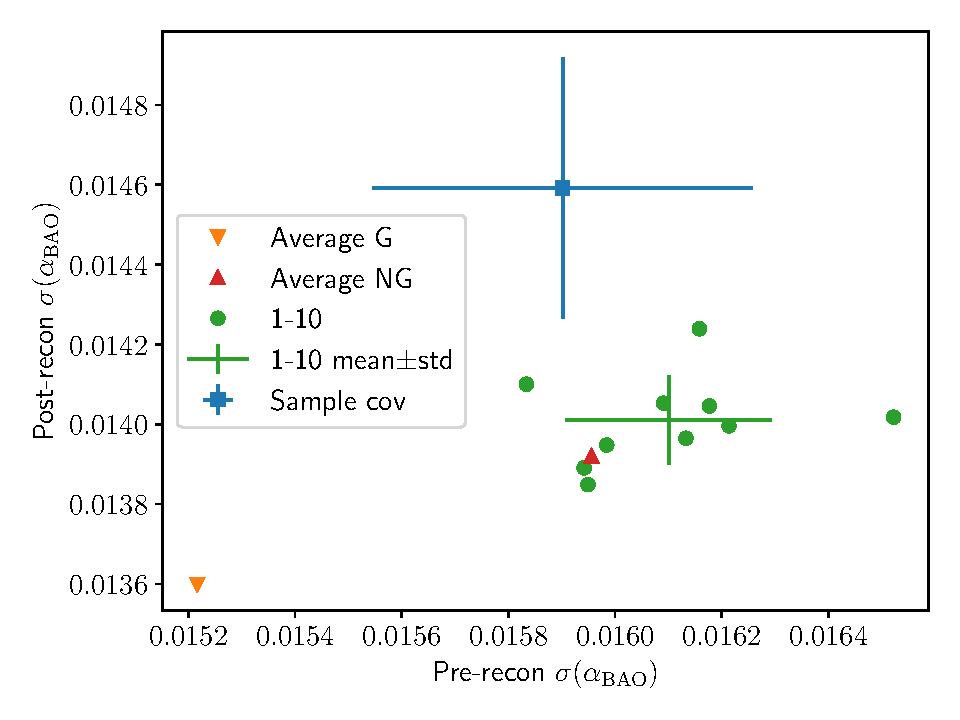
\includegraphics[width=\columnwidth]{img/DESI-M2/sigma_alpha-pre-post.pdf}
\caption[Errorbars on the BAO isotropic scale parameter obtained from different covariances for the \desimtwo{} mocks]{Pre- and post-reconstruction errorbars on $\alpha_{\rm BAO}$ from Fisher forecast plotted against each other.
Compared to the mock-averaged Gaussian run (Average G), the mock-averaged rescaled run (Average NG) and single-mock predictions with rescaling are closer to the sample covariance.
The horizontal (pre-reconstruction) agreement is closer than the vertical (post-reconstruction) one, but even the latter falls within $\approx 2\sigma$.
Note that the range of the axes is quite narrow, comprising only $\approx 9\%$ relative difference in errorbar before reconstruction and $\approx 7\%$ after.}
\label{fig:sigma_alpha-pre-post}
\end{figure}

For the sample covariance, we expect the variance of $C_{S,\alpha\alpha}$ to nearly follow \cref{eq:X-covariance}:
\begin{equation}
\Var \Args{C^{\rm par}_{S,\alpha\alpha}} \approx \frac2{n_S-1} \Arg{C^{\rm par}_{S,\alpha\alpha}}^2
\end{equation}
and therefore the standard deviation of $\sigma(\alpha_{\rm BAO})$ of
\begin{equation} \label{eq:sigma-sigma-alpha}
\sigma\Args{\sigma(\alpha_{\rm BAO})} \approx \frac{\sigma(\alpha_{\rm BAO})}{\sqrt{2(n_S-1)}},
\end{equation}
resulting in relative precision of $2.2\%$.
This has been confirmed in \cref{subsec:stats-validation}.

The resulting errorbar (Fisher) forecasts are provided in \cref{tab:sigma_alpha-pre-post} and also presented as a scatter plot in \cref{fig:sigma_alpha-pre-post}.
We can notice that in any case, the post-recon precision is expected to be higher than pre-recon.
In both pre-recon and post-recon, $\sigma(\alpha_{\rm BAO})$ in the mock-averaged clustering run without shot-noise rescaling are noticeably smaller than predicted from the sample covariance and are brought closer in the rescaled results.
Mock-averaged clustering with fit shot noise and single mock runs gives very similar numbers.
The key conclusion is that single-mock runs are in good agreement with the sample covariance on $\sigma(\alpha_{\rm BAO})$, with a remarkably close match before reconstruction (just fractions of standard deviation) and a difference of $\approx 2$ standard deviation after reconstruction.
This gives assurance that data-based \rascalc{} covariances are on par with mock sample one for isotropic BAO fits.

\section{Application to \desimock{}}
\label{sec:validation-DESI-Y1}

\subsection{DESI DR1 simulations and methods}
\label{sec:simulations-methods}

In this section, we briefly describe the simulations we use and their processing steps.

\subsubsection{Mocks}
\label{sec:mock-types}

In this work, we mainly rely on effective Zel'dovich mocks (\ezmocks{}) \citep{EZmocks,EZmocks2021}.
We use the suite of 1000 catalogs representative of DESI DR1 \citep{KP3s8-Zhao}.
These mocks are more approximate than those relying on full $N$-body simulations.
However, they are fast enough to make a large number of simulations in $6~\ihGpc$ boxes covering the whole volume of DESI DR1 without replications.

For shot-noise rescaling investigation (\cref{sec:shot-noise-rescaling-values}) we also used more realistic \abacussecond{} mocks.
They are based on the {\sc AbacusSummit} suite of $N$-body simulations \citep{AbacusSummit} produced with the {\sc Abacus} code \citep{Abacus-code}.
The halos have been identified with the {\sc CompaSO} halo finder \citep{CompaSO-halo-finder}.
The galaxy catalogs have been produced within halo occupancy distribution (HOD) formalism using the {\sc AbacusHOD} framework \citep{AbacusHOD}.
More details on the suite representing DESI DR1 can be found in \cite{DESI2024.III.KP4}.
These simulations have two disadvantages: only 25 realizations and smaller ($2~\ihGpc$) boxes requiring replications to cover the DESI DR1 volume.

The factors of number and volume are crucial for covariance matrices.
The number of mocks sets the relative precision of the sample covariance estimate, which is the only reference we have for comparison.
By replications, we mean different parts of the final galaxy catalog made from the same part of the original simulation.
These parts can become too strongly correlated and therefore bias the sample covariance estimate.
This motivates our choice of \ezmocks{} for the majority of this work.

\subsubsection{Fiber assignment modeling}
\label{sec:fiber-assignment-models}

An important novel aspect of this work is the application of semi-analytical covariance matrices to mocks that incorporate a model of fiber assignment effects.

We mainly use the approximate algorithm called ``fast fiber assign'' or ``fast fiber assignment'' (FFA) \citep{KP3s11-Sikandar,KP3s6-Bianchi}.
It emulates the DESI fiber assignment algorithm using less computational resources \citep{DESI2024.III.KP4}.

For shot-noise rescaling investigation (\cref{sec:shot-noise-rescaling-values}) we also used the mock realizations of the DESI fiber assignment algorithm.
They involve alternate merged target ledgers, thus the shortcut AMTL \citep{KP3s7-Lasker}.
However, this method is prohibitively slow to process all 1000 \ezmocks{} \citep{DESI2024.III.KP4}.

These fiber assignment algorithms vary in how they assign weights to galaxies and random points to mitigate incompleteness effects.
As discussed in section 5.1 of \cite{KP3s15-Ross}, the DESI assignment completeness can be split into two components, one of which can be modeled by assigning weights to randoms.
However, the FFA algorithm only determines the total assignment completeness per galaxy.
Consequently, the weights per galaxy resulting from FFA have greater variance than for AMTL mocks and the DESI DR1 LSS catalogs.
As we mentioned earlier, different weighting methods for data and random points can affect the shot-noise rescaling values (\cref{eq:shot-noise-approximation}).

Effects of fiber assignment may pose additional challenges to the method because it involves anisotropic pair-wise sampling, depending both on the density of the targets and the number of survey passes in the region \citep{KP3s6-Bianchi}.
We provide the \rascalc{} code with the random catalog and clustering estimate affected by fiber assignment (see the flowchart in \cref{fig:pipeline-jack}), but the expansion leading to \cref{eq:Cov2x2_234_Point_Defs} (and \cref{eq:Cov2x2_234_Point_Defs-jack}) uses the survey-wide correlation function(s) to calculate the ensemble averages of products of overdensities, and the shot-noise rescaling (\cref{eq:shot-noise-approximation}) is also global.
It is challenging to let the correlation function or shot-noise rescaling vary across the survey (with on-sky position or redshift) without complicating the covariance matrix model too much and introducing too many parameters.

Fiber assignment incompleteness might also cause issues with the jackknife.
Ideally, we would like each sub-region to have a distribution of the number of passes representative of the full survey.
This is challenging to achieve, and the current jackknife assignment does not guarantee that.

\subsubsection{Reconstruction}
\label{sec:recon}

We apply the semi-analytical covariance matrix estimators before and after standard BAO reconstruction (pre- and post-recon).
The reconstruction methodology follows the findings of the DESI DR1 optimal reconstruction task force \citep{KP4s3-Chen,KP4s4-Paillas}:
the {\tt RecSym} mode of the {\tt IterativeFFTReconstruction} 
algorithm \citep{recon-fourier-space} from the \pyrecon{} package\footnote{\url{https://github.com/cosmodesi/pyrecon}} with smoothing scale of $15\,\ihMpc$.

\subsubsection{Theoretical modeling and fitting}
\label{sec:theoretical-models-fits}

Our first analysis of interest is DESI 2024 baryon acoustic oscillations \citep{DESI2024.III.KP4}.
We use the same anisotropic (2D) model with BAO power spectrum template and spline-based broadband terms \citep{KP4s2-Chen}.
The fit uses monopole and quadrupole in radial bins spanning $s=48-152\,\ihMpc$.

The second analysis of interest is DESI 2024 full-shape \citep{DESI2024.V.KP5}.
This presents more difficulties because it primarily uses power spectra and the methodology has not been standardized for correlation functions.
Nevertheless, we use similar models relying on the {\tt velocileptors} Lagrangian perturbation theory model \citep{velocileptors-Chen2020,velocileptors-Chen2021,KP5s2-Maus} with maximum freedom and standard prior basis.
Two variants correspond to the power spectrum template choice.
One approach is ``ShapeFit''.
It is a compression method using parametric variations of a single power spectrum template evaluated at the reference cosmology \citep{ShapeFit-Brieden21}.
The other is ``full modeling'', meaning a linear power spectrum from \texttt{CLASS} Boltzmann code \citep{CLASS}.
The fit uses monopole, quadrupole and hexadecapole in radial bins spanning $s=28-152\,\ihMpc$.

These analyses inform our work in two ways.

First, the two fit ranges set our choice of sub-matrices of correlation function multipoles covariances for comparison.
In other words, we restrict the covariance matrices to the multipoles and radial bins used in the fitting.
This gives us an informed choice for smaller sub-matrices to see which parts of the covariance matrix are captured better by the semi-analytic method.

Second, we project the covariance matrices into the parameter spaces of these three models.
We do this with the inverse Fisher matrix as described in \cref{sec:param-space-fisher}.
It is very important to see that the errorbars on physical parameters are predicted reliably through the \rascalc{} covariances, although this analysis may not generalize to alternative models.

We use the \desilike{} package\footnote{\url{https://github.com/cosmodesi/desilike}} for the evaluation of all three models (including polynomial emulators for the full-shape models) and fitting the data.

\subsection{Setup for semi-analytical covariance matrices}
\label{sec:cov-setup}

\begin{table}[tb]
    \centering
    \begin{tabular}{|c|c|c|c|}
        \hline
        Tracer & LRG & ELG & BGS \\
        \hline
        $z$ range & $(0.8, 1.1)$ & $(1.1, 1.6)$ & $(0.1, 0.4)$ \\
        \hline
        Designation in \cite{DESI2024.II.KP3,DESI2024.III.KP4} & {\tt LRG3} & {\tt ELG2} & {\tt BGS} \\
        \hline
        \ezmocks{} snapshot $z$ & 1.1 & 1.325 & 0.2 \\
        \hline
    \end{tabular}
    \caption[Tracers and redshift bins used in \desimock{} validation]{Tracers and redshift bins used in this chapter.
    For LRG and ELG, which have multiple bins unlike BGS, we have selected the densest ones, as shot-noise seems easier to capture with \rascalc{}.
    We did not include the quasars (QSO) for the same reason.
    The snapshot redshifts were used to construct the power spectrum templates.}
    \label{tab:tracers-bins}
\end{table}

We consider three galaxy types (tracers) in three different redshift ranges.
We use luminous red galaxies (LRG) with $z=0.8-1.1$, emission line galaxies (ELG) \citep{ELG.TS.Raichoor.2023} with $z=1.1-1.6$ and magnitude-limited bright galaxy survey (BGS) \citep{BGS.TS.Hahn.2023} with $z=0.1-0.4$.
These correspond to {\tt LRG3}, {\tt ELG2} and {\tt BGS} samples in the main DESI BAO papers \citep{DESI2024.III.KP4,DESI2024.VI.KP7A} respectively.
The summary of tracers and redshift bins is provided in \cref{tab:tracers-bins}.

We apply the data pipeline\footnote{The data scripts are available at \url{https://github.com/cosmodesi/RascalC-scripts/tree/DESI2024/DESI/Y1}, {\tt pre} and {\tt post} directories for single-tracer covariances before and after reconstruction, respectively.
Our analogous single-mock scripts (with only minor differences) are in \url{https://github.com/cosmodesi/RascalC-scripts/tree/DESI2024/DESI/Y1/EZmocks/single}, {\tt pre} and {\tt post} folders.} (\cref{fig:pipeline-jack}) to single mock catalogs, as was done in previous works.
This implies using the random files, full and jackknife correlation function estimates specific to that catalog.
We use 10\footnote{The number is a compromise between getting good statistics and saving computing time.} different realizations of \ezmocks{} to quantify the fluctuations in the semi-analytical results due to realistic random variations in the input quantities.

We process the North and South Galactic Caps (NGC and SGC) separately.
DESI DR1 data has been processed in the same manner.
This allows different shot-noise rescaling values, reflecting different completeness patterns in these parts of DESI DR1.
Then we combine the two covariances into a single matrix for the full survey, assuming the Galactic Caps are uncorrelated\footnote{In the \ezmocks{} NGC and SGC are constructed from separate realizations \cite{KP3s8-Zhao}, so they are independent. As a result, we do not validate this assumption for the data.} (\cref{sec:cov-comb}).

We create the covariance matrices for monopole, quadrupole and hexadecapole in 45 radial bins between 20 and 200~$\ihMpc$ (each 4~$\ihMpc$ wide).
We exclude the $s<20\,\ihMpc$ bins because they impede the convergence of the covariance matrices.
Moreover, we expect the shot-noise rescaling to become inadequate on small scales.

\subsection{Intrinsic tests of the method}
\label{sec:consistency-checks}

Having described the setup for the current \rascalc{} application to \ezmocks{}, we detail the quality checks we perform before comparing the results with the mock sample covariance.

\subsubsection{Intrinsic convergence and computation time}
\label{sec:runtime-intrinsic-convergence}

We have two specific convergence criteria for each \rascalc{} computation.
The first is the eigenvalue test performed by the code on both full and jackknife covariance matrix terms (\cref{eq:Cov2x2_234_Point_Defs_Legendre_Projected,eq:Cov2x2_234_Point_Defs-jack-legendre}).
The desired condition is that the minimal eigenvalue of the 4-point term is larger than minus the minimal eigenvalue of the 2-point term \citep{rascalC}.
The second is the positive definiteness of the final covariance matrix estimate.
We do not use the covariance matrix model that fails either of these tests.

In addition, we have a quantitative measure of convergence without strict thresholds.
As in \cref{subsec:internal-convergence-checks}, we use the $R_{\rm inv}$ comparison measure (\cref{eq:R_inv-definition}) between the different estimates of each \rascalc{} covariance matrix from separate halves of the Monte-Carlo integration samples.
We found several high outliers compared to other mock realizations of the same tracer.

We repeat the computation on the mocks with the convergence issues mentioned before.
Then we post-process the data from the second computation and the data combined from the two computations.
We choose the one that first satisfies the two strict criteria and then gives a lower $R_{\rm inv}$ value.

After this, we find that LRG covariance matrices reached $R_{\rm inv} \le 2.0\%$ convergence within 4 node-hours (512 core-hours\footnote{Hereafter the figure is for the single computation, i.e., effectively twice longer in a few cases. We count physical cores and not hyperthreads. Later profiling also showed a possibility of $\approx 2\times$ improvement by using 64 threads and physical cores instead of 128.}) on the NERSC Perlmutter supercomputer.
The ELG covariance matrices reached $R_{\rm inv} \le 2.9\%$ convergence within 10 node-hours (1280 core-hours).
BGS reached $R_{\rm inv} < 11.5\%$ convergence within 12 node-hours (1536 core-hours).

The computations have become longer relative to \cref{subsec:internal-convergence-checks}, whereas $R_{\rm inv}$ convergence figures have worsened (i.e. increased).
In this previous work, the maximum $R_{\rm inv}$ was $0.63\%$.
The number of 4-point configurations contributing to the sums (\cref{eq:Cov2x2_234_Point_Defs_Legendre_Projected,eq:Cov2x2_234_Point_Defs-jack-legendre}) for LRG NGC or SGC in this work ($2.4\E{12}$) is very close to the analogous number for full LRG in \cref{subsec:internal-convergence-checks} ($2.5\E{12}$), where the sums (\cref{eq:Cov2x2_234_Point_Defs,eq:Cov2x2_234_Point_Defs-jack}) were evaluated for a single angular bin.

The processing of each 4-point configuration becomes longer in Legendre mode.
This can be expected because, as mentioned earlier, a given configuration contributes only to one pair of angular bins, but to all Legendre multipoles.
Other factors, like CPU differences, parallelism efficiency, and a larger number of 3- and 2-point configurations in this work, may also affect the runtimes.

The increase of the $R_{\rm inv}$ convergence measure can be primarily attributed to three times more observables in the covariance matrix.
In this section, we have the same number of radial bins as in \cref{sec:validation-DESI-M2}, but three multipoles instead of only the monopole.
A higher-dimensional covariance matrix requires more configurations sampled for the same relative precision.
Additionally, ELG and especially BGS are more challenging due to the increasing importance of the 4-point term relative to the 3- and 2-point terms.
The more points, the more configurations need to be sampled for the same precision of the term.
Still, the $R_{\rm inv}$ we obtained are significantly smaller than the expected deviation of the mock sample covariance estimate from the true covariance matrix ($R_{\rm inv} \approx 37\%$\footnote{As we show later in \cref{tab:cov-comparison-full}, this number is based on 1000 mock realizations. For a fixed number of samples, the relative precision of the sample covariance also worsens with the number of observables.}).

\subsubsection{Shot-noise rescaling values}
\label{sec:shot-noise-rescaling-values}

\begin{table}[tb]
    \centering
    \begin{tabular}{|c|c|c|c|c|}
\hline
\multirow{2}{*}{$\snrescaling$} & \multicolumn{2}{|c|}{NGC} & \multicolumn{2}{|c|}{SGC} \\
\cline{2-5}
 & Mocks & Data & Mocks & Data \\
\hline
LRG pre-recon & $0.743 \pm 0.012$ & 0.865 & $0.7935 \pm 0.0081$ & 0.953 \\
\hline
LRG post-recon & $0.770 \pm 0.010$ & 0.836 & $0.809 \pm 0.011$ & 0.969 \\
\hline
ELG pre-recon & $0.3757 \pm 0.0043$ & 0.687 & $0.4018 \pm 0.0014$ & 0.718 \\
\hline
ELG post-recon & $0.3789 \pm 0.0044$ & 0.693 & $0.4051 \pm 0.0044$ & 0.737 \\
\hline
BGS pre-recon & $0.792 \pm 0.012$ & 0.855 & $0.8198 \pm 0.0091$ & 0.897 \\
\hline
BGS post-recon & $0.812 \pm 0.012$ & 0.872 & $0.8447 \pm 0.0095$ & 0.934 \\
\hline
    \end{tabular}
    \caption[Shot-noise rescaling values for \desimock{} (one type) and data.]{Shot-noise rescaling values $\snrescaling$ for mocks (10 realizations of FFA \ezmocks{}) and data. % (v1.5 unblinded)
    }
    \label{tab:shot-noise-rescaling}
\end{table}

Our method uses a rescaling of the shot noise contribution to account for differences between the true small-scale contributions and our Gaussian approximation, as we pointed out in \cref{sec:cov-estimation-review}.
After reaching a relatively uniform convergence level in the previous section, we should investigate the values of the shot-noise rescaling parameter.

\cref{tab:shot-noise-rescaling} shows the shot-noise rescaling values obtained for mocks and DESI DR1 data according to the fiducial procedure (\cref{fig:pipeline-jack}).
Interestingly, we find that all the shot-noise rescaling values are smaller than 1;
i.e., the jackknife variations are smaller than predicted by the Gaussian approximation with standard Poisson shot noise.
Previous mock studies \citep[our \cref{subsec:shot-noise-rescaling}]{rascal,rascal-jackknife,rascalC}, on the contrary, obtained shot-noise rescaling values greater than 1.

We also see that the shot-noise rescaling values are significantly lower for mocks than for the data.
The difference is most pronounced for ELGs, which have the lowest shot-noise rescaling values for both mocks and data.
ELGs are also impacted most by the fiber incompleteness effect due to their lower priority compared to other dark-time targets, LRG and QSO \cite{ELG.TS.Raichoor.2023}.
This suggests that the low shot-noise rescaling is related to fiber assignment.

To test whether fiber assignment is the main cause for low and different shot-noise rescaling values, we have performed additional \rascalc{} computations using more realistic \abacus{} mocks and the DESI fiber assignment algorithm (AMTL).
We only used one realization for LRG and ELG in each case to save computing time.

\begin{table}[tb!]
    \centering
    \begin{tabular}{|c|c|c|c|c|c|c|}
\hline
\multirow{2}{*}{$\snrescaling$} & \multirow{2}{*}{Data} & \multicolumn{2}{|c|}{AMTL (correct)} & \multicolumn{2}{|c|}{FFA (approximate)} & Complete \\
\cline{3-7}
 &  & \abacus{} & \ezmocks{} & \abacus{} & \ezmocks{} & \abacus{} \\
\hline
LRG NGC & 0.865 & 0.845 & 0.886 & 0.721 & 0.758 & 0.934 \\
\hline
LRG SGC & 0.953 & 0.954 & 0.961 & 0.781 & 0.784 & 0.962 \\
\hline
ELG NGC & 0.687 & 0.649 & 0.672 & 0.378 & 0.380 & 0.965 \\
\hline
ELG SGC & 0.718 & 0.707 & 0.744 & 0.405 & 0.403 & 0.968 \\
\hline
    \end{tabular}
    \caption[Shot-noise rescaling values for the data and two different types of mocks with two different fiber assignment models]{Shot-noise rescaling values $\alpha_{\rm SN}$ (before reconstruction) for the data and two different types of mocks (\cref{sec:mock-types}) with two different fiber assignment models (\cref{sec:fiber-assignment-models}).
    ``Complete'' designates mocks before fiber assignment.
    We use a single mock realization for each category.}
    \label{tab:shot-noise-rescaling-ffa-altmtl}
\end{table}

\cref{tab:shot-noise-rescaling-ffa-altmtl} shows the shot-noise rescaling values for data and different mocks (\abacus{} or \ezmocks{}) with different fiber assignment models (FFA or AMTL).
We also include an \abacus{} mock before fiber assignment (``complete'').
We see that the fiber assignment modeling method makes a bigger difference than the type of mocks.
The approximate fast fiber assignment gives the lowest shot-noise rescaling values.
The DESI fiber assignment algorithm applied to the mocks (AMTL) gives $\alpha_{\rm SN}$ very similar to the data.
The complete \abacus{} mocks have larger shot-noise rescaling values than data and fiber-assigned mocks.
This confirms the fiber assignment as a key factor affecting the $\alpha_{\rm SN}$ parameter.

The discrepancy in shot-noise rescaling values also raises concerns about the quality of approximations in the FFA algorithm.
However, of all the mock types, only \ezmocks{} processed with FFA are numerous enough for a precise sample covariance estimate.
Therefore, we continue using them in the remainder of this paper.

\begin{table}[tb!]
    \centering
    \begin{tabular}{|c|c|c|c|c|}
\hline
\multirow{2}{*}{$\snrescaling$} & \multicolumn{2}{|c|}{NGC} & \multicolumn{2}{|c|}{SGC} \\
\cline{2-5}
 & Jackknife & Mock sample & Jackknife & Mock sample \\
\hline
LRG pre & $0.743 \pm 0.012$ & $0.7417 \pm 0.0038$ & $0.7935 \pm 0.0081$ & $0.7906 \pm 0.0045$ \\
\hline
LRG post & $0.770 \pm 0.010$ & $0.7446 \pm 0.0029$ & $0.809 \pm 0.011$ & $0.7945 \pm 0.0032$ \\
\hline
ELG pre & $0.3757 \pm 0.0043$ & $0.3757 \pm 0.0013$ & $0.4018 \pm 0.0014$ & $0.4077 \pm 0.0016$ \\
\hline
ELG post & $0.3789 \pm 0.0044$ & $0.3751 \pm 0.0013$ & $0.4051 \pm 0.0044$ & $0.4067 \pm 0.0017$ \\
\hline
BGS pre & $0.792 \pm 0.012$ & $0.7916 \pm 0.0068$ & $0.8198 \pm 0.0091$ & $0.827 \pm 0.014$ \\
\hline
BGS post & $0.812 \pm 0.012$ & $0.8148 \pm 0.0070$ & $0.8447 \pm 0.0095$ & $0.844 \pm 0.013$ \\
\hline
    \end{tabular}
    \caption{Shot-noise rescaling values for the single-mock runs calibrated on jackknife (\cref{fig:pipeline-jack}) and mock sample covariances (\cref{fig:pipeline-mocks}).}
    \label{tab:shot-noise-rescaling-jack-mocks}
\end{table}

We performed the final consistency tests of the shot-noise optimization procedure in light of the concerns about fiber assignment and jackknife discussed in \cref{sec:fiber-assignment-models}.
We optimized the shot-noise rescaling based on mock sample covariance (the process is shown schematically in \cref{fig:pipeline-mocks}).
We show the resulting values along with the baseline, jackknife-based ones in \cref{tab:shot-noise-rescaling-jack-mocks}, and find them very close for all cases.
In other words, calibration of shot-noise rescaling on jackknives still brings us close to an optimal fit on the mocks.
With that, we have decided to proceed further with the validation process using the jackknife-calibrated shot-noise rescaling values.
This will show how close this nearly optimal fit is to the mock sample covariance.

\subsection{Comparison between semi-analytical and mock sample covariance matrices}
\label{sec:cov-comparison-results}

Thus, we reach the last validation part: comparison of the semi-analytical covariances obtained from single mock catalogs with the mock sample covariance matrices.
We compute three similarity measures (\cref{subsec:comparison-measures}) between these covariance matrices for each tracer before and after standard BAO reconstruction (pre- and post-recon).
Instead of presenting 10 numbers (corresponding to each \rascalc{} realization) for each case in the paper, we provide their mean and standard deviation.
The full set of comparison measure values is available in the supplementary material\footnote{\supplementarylink{}}.
We also provide the ``perfect'' reference row, listing the statistical properties of the similarity measures between the true covariance and a mock sample covariance matrix based on their dimension (also obtained in \cref{subsec:comparison-measures}).

We note that the standard deviation in the ``perfect'' row is different and independent from the others.
The ``perfect'' standard deviation characterizes the distribution of the random difference between the sample covariance estimate from 1000 realizations and the true covariance.
In each other row (tracer + pre- or post-recon combination), the sample covariance estimate is fixed, and the standard deviation describes the scatter resulting from 10 different \rascalc{} covariance realizations.

Ideally, every \rascalc{} covariance matrix would be consistent with the true covariance.
To see whether this is the case, we compute the difference between each comparison measure for each \rascalc{} covariance realization and the corresponding ``perfect'' mean in ``perfect'' standard deviations.
We summarize the 10 resulting quantities by the mean and standard deviation as well, and provide them below the summary of the similarity measure itself.
This sets the common structure for all tables in this section (i.e., \cref{tab:cov-comparison-full,tab:cov-comparison-shape-range,tab:cov-comparison-BAO-range,tab:cov-comparison-BAO-parameters,tab:cov-comparison-ShapeFit-parameters,tab:cov-comparison-direct-fit-parameters}.).

\subsubsection{Observables}
\label{sec:cov-comparison-obs}

We begin with the covariances for correlation function multipoles, in other words, in the space of observables. 

\begin{table}[tb]
\centering
\begin{tabular}{|c|c|c|c|}
\hline
 & $D_{\rm KL} ({\bf C}_R^{-1}, {\bf C}_S)$ & $R_{\rm inv} ({\bf C}_R^{-1}, {\bf C}_S)$ & $\chi^2_{\rm red} ({\bf C}_R^{-1}, {\bf C}_S)$ \\
\hline
Perfect & $4.817 \pm 0.070$ & $0.3690 \pm 0.0031$ & $1.0000 \pm 0.0039$ \\
\hline
\multirow{2}{*}{LRG pre-recon} & $4.856 \pm 0.029$ & $0.3678 \pm 0.0049$ & $0.989 \pm 0.016$ \\
 & ($0.55 \pm 0.41$)$\sigma$ & ($-0.4 \pm 1.6$)$\sigma$ & ($-2.7 \pm 4.1$)$\sigma$ \\
\hline
\multirow{2}{*}{LRG post-recon} & $4.977 \pm 0.050$ & $0.3581 \pm 0.0034$ & $0.957 \pm 0.014$ \\
 & ($2.27 \pm 0.70$)$\sigma$ & ($-3.5 \pm 1.1$)$\sigma$ & ($-11.3 \pm 3.6$)$\sigma$ \\
\hline
\multirow{2}{*}{ELG pre-recon} & $4.811 \pm 0.024$ & $0.3700 \pm 0.0055$ & $1.000 \pm 0.015$ \\
 & ($-0.09 \pm 0.34$)$\sigma$ & ($0.3 \pm 1.8$)$\sigma$ & ($0.1 \pm 3.8$)$\sigma$ \\
\hline
\multirow{2}{*}{ELG post-recon} & $5.001 \pm 0.018$ & $0.3701 \pm 0.0042$ & $0.986 \pm 0.012$ \\
 & ($2.61 \pm 0.26$)$\sigma$ & ($0.4 \pm 1.4$)$\sigma$ & ($-3.6 \pm 3.1$)$\sigma$ \\
\hline
\multirow{2}{*}{BGS pre-recon} & $5.129 \pm 0.052$ & $0.3824 \pm 0.0081$ & $0.997 \pm 0.016$ \\
 & ($4.43 \pm 0.73$)$\sigma$ & ($4.4 \pm 2.6$)$\sigma$ & ($-0.8 \pm 4.2$)$\sigma$ \\
\hline
\multirow{2}{*}{BGS post-recon} & $5.177 \pm 0.077$ & $0.3810 \pm 0.0079$ & $0.994 \pm 0.016$ \\
 & ($5.1 \pm 1.1$)$\sigma$ & ($3.9 \pm 2.6$)$\sigma$ & ($-1.4 \pm 4.1$)$\sigma$ \\
\hline
\end{tabular}
\caption[Full observable-space comparison of \rascalc{} covariances with the \desimock{} sample covariances]{Summary of full observable-space comparison of \rascalc{} covariances with the sample covariances (135 bins, $s=20-200~\ihMpc$, monopole, quadrupole and hexadecapole).}
\label{tab:cov-comparison-full}
\end{table}

\cref{tab:cov-comparison-full} shows the comparison measures for the full covariance matrices, covering $s=20-200~\ihMpc$ radial bins for all three multipoles.
We can see that some \rascalc{} results deviate significantly from the ``perfect'' (i.e., the true covariance behavior).
We remind that the KL divergence and $R_{\rm inv}$ accumulate deviations in all ``directions''.
The KL divergences exceed the ideal expectation value by nearly $3\sigma$ for LRG and ELG post-recon, whereas for BGS they are even further from perfect.
$R_{\rm inv}$ values are high with a larger scatter for BGS.
In the reduced chi-squared, which captures the overall ``scaling'' with higher accuracy, the mean values for the \rascalc{} runs are shifted significantly for LRG and ELG post-recon, and the mock-to-mock scatter is high in all the cases.

\begin{table}[tb]
\centering
\begin{tabular}{|c|c|c|c|}
\hline
 & $D_{\rm KL} ({\bf C}_R^{-1}, {\bf C}_S)$ & $R_{\rm inv} ({\bf C}_R^{-1}, {\bf C}_S)$ & $\chi^2_{\rm red} ({\bf C}_R^{-1}, {\bf C}_S)$ \\
\hline
Perfect & $2.260 \pm 0.049$ & $0.3067 \pm 0.0036$ & $1.0000 \pm 0.0046$ \\
\hline
\multirow{2}{*}{LRG pre-recon} & $2.307 \pm 0.022$ & $0.3056 \pm 0.0037$ & $0.983 \pm 0.016$ \\
 & ($0.99 \pm 0.46$)$\sigma$ & ($-0.3 \pm 1.0$)$\sigma$ & ($-3.7 \pm 3.4$)$\sigma$ \\
\hline
\multirow{2}{*}{LRG post-recon} & $2.333 \pm 0.027$ & $0.2998 \pm 0.0024$ & $0.960 \pm 0.014$ \\
 & ($1.52 \pm 0.56$)$\sigma$ & ($-1.93 \pm 0.68$)$\sigma$ & ($-8.7 \pm 3.0$)$\sigma$ \\
\hline
\multirow{2}{*}{ELG pre-recon} & $2.2578 \pm 0.0095$ & $0.3050 \pm 0.0044$ & $0.995 \pm 0.014$ \\
 & ($-0.04 \pm 0.20$)$\sigma$ & ($-0.5 \pm 1.2$)$\sigma$ & ($-1.0 \pm 3.1$)$\sigma$ \\
\hline
\multirow{2}{*}{ELG post-recon} & $2.292 \pm 0.013$ & $0.3044 \pm 0.0033$ & $0.987 \pm 0.012$ \\
 & ($0.67 \pm 0.28$)$\sigma$ & ($-0.65 \pm 0.93$)$\sigma$ & ($-2.8 \pm 2.6$)$\sigma$ \\
\hline
\multirow{2}{*}{BGS pre-recon} & $2.414 \pm 0.025$ & $0.3140 \pm 0.0066$ & $0.987 \pm 0.016$ \\
 & ($3.18 \pm 0.52$)$\sigma$ & ($2.0 \pm 1.9$)$\sigma$ & ($-2.7 \pm 3.4$)$\sigma$ \\
\hline
\multirow{2}{*}{BGS post-recon} & $2.479 \pm 0.038$ & $0.3202 \pm 0.0065$ & $0.993 \pm 0.016$ \\
 & ($4.52 \pm 0.78$)$\sigma$ & ($3.8 \pm 1.8$)$\sigma$ & ($-1.5 \pm 3.4$)$\sigma$ \\
\hline
\end{tabular}
\caption[Observable-space comparison of \rascalc{} covariances with the \desimock{} sample covariances restricted to the range of ShapeFit and full modeling fits]{Summary of observable-space comparison of \rascalc{} covariances with the sample covariances restricted to the range of ShapeFit and full modeling fit (93 bins, $s=28-152~\ihMpc$, monopole, quadrupole and hexadecapole).}
\label{tab:cov-comparison-shape-range}
\end{table}

We continue the comparisons in \cref{tab:cov-comparison-shape-range}, now cutting the range to $s=28-152~\ihMpc$ as is common for full-shape fits (ShapeFit and direct).
The KL divergences and $R_{\rm inv}$ become more consistent with the perfect reference cases for LRG and ELG, but remain high for BGS.
The scaling difference (in reduced chi-squared) remains similar.

\begin{table}[tb]
\centering
\begin{tabular}{|c|c|c|c|}
\hline
 & $D_{\rm KL} ({\bf C}_R^{-1}, {\bf C}_S)$ & $R_{\rm inv} ({\bf C}_R^{-1}, {\bf C}_S)$ & $\chi^2_{\rm red} ({\bf C}_R^{-1}, {\bf C}_S)$ \\
\hline
Perfect & $0.702 \pm 0.027$ & $0.2303 \pm 0.0046$ & $1.0000 \pm 0.0062$ \\
\hline
\multirow{2}{*}{LRG pre-recon} & $0.763 \pm 0.014$ & $0.2351 \pm 0.0023$ & $0.982 \pm 0.016$ \\
 & ($2.29 \pm 0.54$)$\sigma$ & ($1.04 \pm 0.49$)$\sigma$ & ($-2.9 \pm 2.6$)$\sigma$ \\
\hline
\multirow{2}{*}{LRG post-recon} & $0.732 \pm 0.013$ & $0.2281 \pm 0.0019$ & $0.964 \pm 0.015$ \\
 & ($1.14 \pm 0.50$)$\sigma$ & ($-0.48 \pm 0.40$)$\sigma$ & ($-5.7 \pm 2.3$)$\sigma$ \\
\hline
\multirow{2}{*}{ELG pre-recon} & $0.7195 \pm 0.0083$ & $0.2317 \pm 0.0039$ & $0.999 \pm 0.015$ \\
 & ($0.65 \pm 0.31$)$\sigma$ & ($0.30 \pm 0.86$)$\sigma$ & ($-0.2 \pm 2.4$)$\sigma$ \\
\hline
\multirow{2}{*}{ELG post-recon} & $0.6903 \pm 0.0088$ & $0.2278 \pm 0.0029$ & $0.995 \pm 0.012$ \\
 & ($-0.45 \pm 0.33$)$\sigma$ & ($-0.54 \pm 0.62$)$\sigma$ & ($-0.8 \pm 1.9$)$\sigma$ \\
\hline
\multirow{2}{*}{BGS pre-recon} & $0.796 \pm 0.021$ & $0.2419 \pm 0.0079$ & $0.982 \pm 0.018$ \\
 & ($3.54 \pm 0.78$)$\sigma$ & ($2.5 \pm 1.7$)$\sigma$ & ($-2.8 \pm 2.8$)$\sigma$ \\
\hline
\multirow{2}{*}{BGS post-recon} & $0.777 \pm 0.031$ & $0.2462 \pm 0.0090$ & $1.011 \pm 0.017$ \\
 & ($2.8 \pm 1.2$)$\sigma$ & ($3.4 \pm 1.9$)$\sigma$ & ($1.8 \pm 2.7$)$\sigma$ \\
\hline
\end{tabular}
\caption[Observable-space comparison of \rascalc{} covariances with the \desimock{} sample covariances restricted to the range of BAO fits]{Summary of observable-space comparison of \rascalc{} covariances with the sample covariances restricted to the range of BAO fits (52 bins, $s=48-152~\ihMpc$, monopole and quadrupole).}
\label{tab:cov-comparison-BAO-range}
\end{table}

We perform the final set of observable-space comparisons in \cref{tab:cov-comparison-BAO-range}, further restricting the range to $s=48-152~\ihMpc$ and using only monopole and quadrupole, without hexadecapole.
We do not see significant consistency changes from the previous case.

We note that the abovementioned differences are relatively small.
In the reduced chi-squared, they are at most $(4.3 \pm 1.4)\%$ for LRG post-recon in the widest range, and in $R_{\rm inv}$ -- no more than a percent or two on top of $23-37\%$ caused by the finite sample size.
We should ask whether we trust the realism of the mocks to such a high level in all aspects of the correlation function multipoles.
Moreover, for the real survey, matching the clustering between data and simulations will become an additional issue for mocks.
On the other hand, our \rascalc{} computations use the correlation function measured directly from single mock catalogs similar to real data.
Thus, we conclude that the semi-analytic method's performance is very compelling.

\subsubsection{Model parameters}
\label{sec:cov-comparison-param}

We proceed to project the covariance matrices (as described in \cref{sec:param-space-fisher}) to the parameters of the models listed in \cref{sec:theoretical-models-fits}.

We use the same model Jacobian (\cref{eq:model-jacobian}) for projecting \rascalc{} covariances (\cref{eq:parameter-covariance-rascalc}) and the mock sample covariances (\cref{eq:parameter-covariance-sample}) into the parameter space.
We compute the partial derivatives at the best fit of each model to the mean clustering of all the available mocks for each galaxy type.
Since BAO reconstruction changes clustering, we compute separate Jacobians before and after reconstruction.
We use the mock sample covariance matrix in this fit.
Using different Jacobian matrices for each covariance matrix would complicate the comparison.

A more thorough investigation of the covariance matrix's impact on the model fits is presented in the companion paper \citep{KP4s6-Forero-Sanchez}.
They perform fits to each mock clustering using different covariance matrices (mock sample and semi-analytical) and compare the resulting best parameter values as well as errorbar estimates.
On the flip side, with such a detailed approach \cite{KP4s6-Forero-Sanchez} can not test multiple \rascalc{} single-mock covariances.

\subsubsection{BAO}
\label{sec:cov-comparison-bao-param}

\begin{table}[tb]
\centering
\begin{tabular}{|c|c|c|c|}
\hline
 & $D_{\rm KL} ({\bf C}_R^{-1}, {\bf C}_S)$ & $R_{\rm inv} ({\bf C}_R^{-1}, {\bf C}_S)$ & $\chi^2_{\rm red} ({\bf C}_R^{-1}, {\bf C}_S)$ \\
\hline
Perfect & $0.0015 \pm 0.0012$ & $0.051 \pm 0.021$ & $1.000 \pm 0.032$ \\
\hline
\multirow{2}{*}{LRG pre-recon} & $0.00103 \pm 0.00066$ & $0.042 \pm 0.014$ & $0.960 \pm 0.014$ \\
 & ($-0.39 \pm 0.53$)$\sigma$ & ($-0.39 \pm 0.67$)$\sigma$ & ($-1.27 \pm 0.45$)$\sigma$ \\
\hline
\multirow{2}{*}{LRG post-recon} & $0.00110 \pm 0.00026$ & $0.0458 \pm 0.0051$ & $0.9734 \pm 0.0098$ \\
 & ($-0.32 \pm 0.21$)$\sigma$ & ($-0.23 \pm 0.24$)$\sigma$ & ($-0.84 \pm 0.31$)$\sigma$ \\
\hline
\multirow{2}{*}{ELG pre-recon} & $0.00069 \pm 0.00036$ & $0.0367 \pm 0.0093$ & $1.033 \pm 0.010$ \\
 & ($-0.66 \pm 0.29$)$\sigma$ & ($-0.65 \pm 0.44$)$\sigma$ & ($1.04 \pm 0.32$)$\sigma$ \\
\hline
\multirow{2}{*}{ELG post-recon} & $0.00078 \pm 0.00045$ & $0.037 \pm 0.012$ & $0.967 \pm 0.012$ \\
 & ($-0.59 \pm 0.37$)$\sigma$ & ($-0.63 \pm 0.55$)$\sigma$ & ($-1.05 \pm 0.38$)$\sigma$ \\
\hline
\multirow{2}{*}{BGS pre-recon} & $0.0042 \pm 0.0016$ & $0.088 \pm 0.015$ & $0.915 \pm 0.014$ \\
 & ($2.2 \pm 1.3$)$\sigma$ & ($1.74 \pm 0.71$)$\sigma$ & ($-2.68 \pm 0.46$)$\sigma$ \\
\hline
\multirow{2}{*}{BGS post-recon} & $0.00027 \pm 0.00024$ & $0.0213 \pm 0.0093$ & $0.992 \pm 0.013$ \\
 & ($-1.00 \pm 0.19$)$\sigma$ & ($-1.38 \pm 0.44$)$\sigma$ & ($-0.24 \pm 0.40$)$\sigma$ \\
\hline
\end{tabular}
\caption[Parameter-space comparison of \rascalc{} covariances with the \desimock{} sample covariances projected to the BAO fit parameters]{Summary of parameter-space comparison of \rascalc{} covariances with the sample covariances projected to the BAO fit parameters, $\alphaiso$ and $\alphaap$.}
\label{tab:cov-comparison-BAO-parameters}
\end{table}

In \cref{tab:cov-comparison-BAO-parameters} we compare the covariances projected to the BAO parameters, the scaling parameters $\alphaiso$ and $\alphaap$\footnote{Because we use Fisher matrix formalism, the covariance matrices projected for $\alpha_\parallel$ and $\alpha_\perp$ should have the same comparison measures.}.
The comparison measures look consistent with the perfect reference case.
The most significant deviations are seen in BGS pre-recon: both the KL divergence and $R_{\rm inv}$ are high, while the reduced chi-squared is almost 3 sigma low on average (meaning that the \rascalc{} covariance is ``larger'' than the mock sample one).
The mock-to-mock scatter in \rascalc{} results is always lower than the noise expected from the finite mock sample size.

\begin{figure}[tb]
\centering
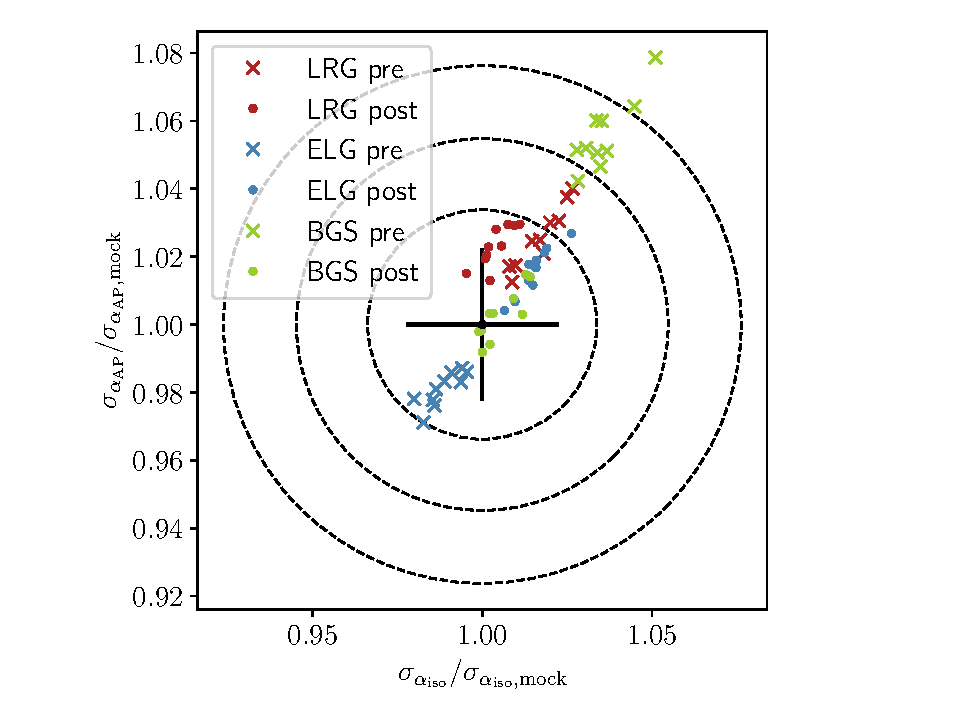
\includegraphics[width=\textwidth]{img/DESI-Y1/normalized_errorbars_bao.pdf}
\caption[Comparison of the projected errorbars for the BAO scale parameters for \desimock{}]{Comparison of the projected errorbars for the BAO scale parameters, normalized to the values obtained from the mock sample covariance.
The cross shows one-dimensional relative precisions ($\qty(2\qty(n_S-1))^{-1/2} \approx 2.2\%$, \cref{eq:sigma-sigma-alpha}) following from the \ezmocks{} sample size ($n_S=1000$), and the dashed ellipses approximately correspond to two-dimensional 68\%, 95\% and 99.7\% confidence regions in this 2D space of errorbars.
Here, the correlation of errorbars is ignored; it varies in different cases but is too small to notice ($\lesssim 0.04$).}
\label{fig:BAO-errorbars}
\end{figure}

We have also plotted the errorbars on $\alphaiso$ and $\alphaap$ against each other in \cref{fig:BAO-errorbars}.
They corroborate \cref{tab:cov-comparison-BAO-parameters}.
Almost all deviations are within the 99.7\% contour.
The only exceptions are two BGS pre-recon realizations.
However, we note that these plots do not show the covariance of the parameters, which is taken into account with KL divergence and $R_{\rm inv}$.

\subsubsection{Full shape: ShapeFit and full modeling}
\label{sec:cov-comparison-fullshape-param}

\begin{table}[tb]
\centering
\begin{tabular}{|c|c|c|c|}
\hline
 & $D_{\rm KL} ({\bf C}_R^{-1}, {\bf C}_S)$ & $R_{\rm inv} ({\bf C}_R^{-1}, {\bf C}_S)$ & $\chi^2_{\rm red} ({\bf C}_R^{-1}, {\bf C}_S)$ \\
\hline
Perfect & $0.0050 \pm 0.0023$ & $0.069 \pm 0.016$ & $1.000 \pm 0.022$ \\
\hline
\multirow{2}{*}{LRG pre-recon} & $0.0059 \pm 0.0023$ & $0.073 \pm 0.013$ & $0.969 \pm 0.020$ \\
 & ($0.4 \pm 1.0$)$\sigma$ & ($0.25 \pm 0.81$)$\sigma$ & ($-1.39 \pm 0.89$)$\sigma$ \\
\hline
\multirow{2}{*}{LRG post-recon} & $0.00739 \pm 0.00087$ & $0.0840 \pm 0.0052$ & $0.984 \pm 0.022$ \\
 & ($1.06 \pm 0.39$)$\sigma$ & ($0.95 \pm 0.33$)$\sigma$ & ($-0.73 \pm 0.98$)$\sigma$ \\
\hline
\multirow{2}{*}{ELG pre-recon} & $0.0063 \pm 0.0029$ & $0.078 \pm 0.015$ & $1.005 \pm 0.027$ \\
 & ($0.6 \pm 1.3$)$\sigma$ & ($0.59 \pm 0.94$)$\sigma$ & ($0.2 \pm 1.2$)$\sigma$ \\
\hline
\multirow{2}{*}{ELG post-recon} & $0.0029 \pm 0.0013$ & $0.052 \pm 0.011$ & $0.999 \pm 0.017$ \\
 & ($-0.95 \pm 0.58$)$\sigma$ & ($-1.06 \pm 0.68$)$\sigma$ & ($-0.06 \pm 0.78$)$\sigma$ \\
\hline
\multirow{2}{*}{BGS pre-recon} & $0.0071 \pm 0.0030$ & $0.083 \pm 0.019$ & $0.996 \pm 0.031$ \\
 & ($0.9 \pm 1.3$)$\sigma$ & ($0.9 \pm 1.2$)$\sigma$ & ($-0.2 \pm 1.4$)$\sigma$ \\
\hline
\multirow{2}{*}{BGS post-recon} & $0.0067 \pm 0.0027$ & $0.080 \pm 0.017$ & $0.992 \pm 0.030$ \\
 & ($0.7 \pm 1.2$)$\sigma$ & ($0.7 \pm 1.1$)$\sigma$ & ($-0.3 \pm 1.3$)$\sigma$ \\
\hline
\end{tabular}
\caption[Parameter-space comparison of \rascalc{} covariances with the \desimock{} sample covariances projected to the ShapeFit parameters]{Summary of parameter-space comparison of \rascalc{} covariances with the sample covariances projected to the ShapeFit parameters: $\alphaiso$, $\alphaap$, $dm$ and $df$.}
\label{tab:cov-comparison-ShapeFit-parameters}
\end{table}

\cref{tab:cov-comparison-ShapeFit-parameters} shows the comparison measures for the covariances projected to the ShapeFit parameters: $\alphaiso$, $\alphaap$, $dm$ and $df$.
We do not see significant statistical deviations from the perfect case.
This is the only case when BGS (both pre- and post-recon) are not particularly far from the reference.
The mock-to-mock scatter in \rascalc{} results is smaller than or comparable with the noise in the sample covariances.

\begin{figure}[tb]
\centering
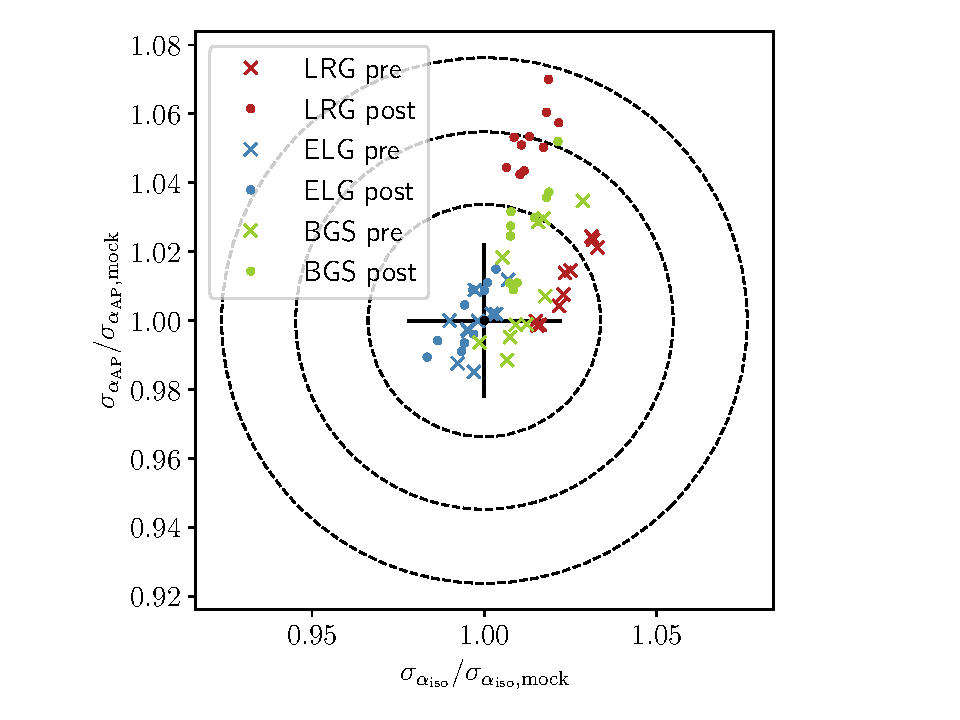
\includegraphics[width=\textwidth]{img/DESI-Y1/normalized_errorbars_shapefit.pdf}
\caption[Comparison of the projected errorbars for the BAO scale parameters for \desimock{} from ShapeFit]{Same as \cref{fig:BAO-errorbars} but with errorbars for the scale parameters following from ShapeFit.}
\label{fig:shapefit-scale-errorbars}
\end{figure}

Additionally, in \cref{fig:shapefit-scale-errorbars} we compare the projected errorbars for the scaling parameters, $\alphaiso$ and $\alphaap$.
All the points fall within the 99.7\% confidence region in this 2D space, although the other parameters and cross-correlations are ignored in this picture, unlike in \cref{tab:cov-comparison-ShapeFit-parameters}.

\begin{table}[tb]
\centering
\begin{tabular}{|c|c|c|c|}
\hline
 & $D_{\rm KL} ({\bf C}_R^{-1}, {\bf C}_S)$ & $R_{\rm inv} ({\bf C}_R^{-1}, {\bf C}_S)$ & $\chi^2_{\rm red} ({\bf C}_R^{-1}, {\bf C}_S)$ \\
\hline
Perfect & $0.0050 \pm 0.0023$ & $0.069 \pm 0.016$ & $1.000 \pm 0.022$ \\
\hline
\multirow{2}{*}{LRG pre-recon} & $0.0099 \pm 0.0034$ & $0.093 \pm 0.014$ & $0.951 \pm 0.020$ \\
 & ($2.2 \pm 1.5$)$\sigma$ & ($1.50 \pm 0.89$)$\sigma$ & ($-2.20 \pm 0.91$)$\sigma$ \\
\hline
\multirow{2}{*}{LRG post-recon} & $0.00360 \pm 0.00068$ & $0.0584 \pm 0.0055$ & $0.976 \pm 0.016$ \\
 & ($-0.63 \pm 0.30$)$\sigma$ & ($-0.66 \pm 0.35$)$\sigma$ & ($-1.08 \pm 0.71$)$\sigma$ \\
\hline
\multirow{2}{*}{ELG pre-recon} & $0.0061 \pm 0.0013$ & $0.0783 \pm 0.0094$ & $1.013 \pm 0.024$ \\
 & ($0.48 \pm 0.60$)$\sigma$ & ($0.59 \pm 0.59$)$\sigma$ & ($0.6 \pm 1.1$)$\sigma$ \\
\hline
\multirow{2}{*}{ELG post-recon} & $0.0033 \pm 0.0014$ & $0.055 \pm 0.011$ & $0.985 \pm 0.016$ \\
 & ($-0.75 \pm 0.60$)$\sigma$ & ($-0.85 \pm 0.72$)$\sigma$ & ($-0.68 \pm 0.72$)$\sigma$ \\
\hline
\multirow{2}{*}{BGS pre-recon} & $0.0101 \pm 0.0073$ & $0.099 \pm 0.040$ & $1.013 \pm 0.035$ \\
 & ($2.3 \pm 3.2$)$\sigma$ & ($1.9 \pm 2.5$)$\sigma$ & ($0.6 \pm 1.5$)$\sigma$ \\
\hline
\multirow{2}{*}{BGS post-recon} & $0.0083 \pm 0.0045$ & $0.090 \pm 0.027$ & $1.003 \pm 0.035$ \\
 & ($1.5 \pm 2.0$)$\sigma$ & ($1.3 \pm 1.7$)$\sigma$ & ($0.1 \pm 1.5$)$\sigma$ \\
\hline
\end{tabular}
\caption[Parameter-space comparison of \rascalc{} covariances with the \desimock{} sample covariances projected to the full modeling parameters]{Summary of parameter-space comparison of \rascalc{} covariances with the sample covariances projected to the full modeling parameters: $h$, $\omega_{\rm cdm}$, $\omega_b$ and $\log A_s$.}
\label{tab:cov-comparison-direct-fit-parameters}
\end{table}

Finally, in \cref{tab:cov-comparison-direct-fit-parameters} we provide the comparison results for the covariances projected to the full modeling parameters, $h$, $\omega_{\rm cdm}$, $\omega_b$ and $\log A_s$.
We see deviations exceeding 3 sigma in most of the measures for LRG pre-recon and BGS; LRG post-recon and ELG look consistent.
Still, the differences we see are at a few percent level, and may be caused by the limited realism of the mocks.

\section{Conclusions}
\label{sec:conclusion-rascalc}

We present and validate the DESI DR1 pipeline for the semi-analytical covariance matrices of the galaxy 2-point correlation functions on realistic mock catalogs, including a model of fiber assignment.

We develop a streamlined procedure for the estimation of the semi-analytical covariance matrices for Legendre moments of the 2PCF in separation bins with the \rascalc{} code \citep{rascalC}.
The previous implementation \citep{rascalC-legendre-3} required an additional computation with angular bins to mimic the non-Gaussian effects by calibrating the shot-noise rescaling value on the jackknife covariance matrix estimate.
Now we can perform this calibration together with the construction of the covariance model for Legendre moments.
This allowed for more efficient massive production of covariance matrices for all the tracers, redshift bins, and galactic caps of DESI DR1 galaxies and quasars data.

Importantly, we reconsidered the methods for covariance matrix comparison, paying great attention to their meaning, interpretation, and noise stemming from mock sample variance.
We have also discussed the implications of split random-random counts computation and made a slight modification to the formalism to cover the reconstructed 2PCF estimates.

We have applied the selected approaches to the validation of \rascalc{} on single \themock{} catalogs (using their individual clustering measurements and shifted random catalogs after reconstruction), each representing a reasonable proxy for \desimtwo{} data, by comparison with full mock sample covariance.
We find a close agreement (maximum deviation $\approx 2.2\sigma$) with a perfect case, although much of this deviation is due to scatter in \rascalc{} results.
The preceding discussion about the interpretations of the metrics, focusing on a smaller number of observables and even fewer parameters, allowed us to obtain a clearer quantitative assessment of the precision and accuracy of \rascalc{} results than in previous works.
One should keep in mind that the mocks are approximate, and this can partially account for the imperfection of the match with the reference statistics.

Focusing on the errorbar of the BAO scale, we found a very close, percent-level agreement with the sample covariance from mocks.
It is on par with the accuracy that a set of $\approx 1000$ simulations can provide.
The number of available mocks thus limits the precision of the validation at the current level.

In the full measurement space before reconstruction, using the shot-noise rescaling is particularly clearly beneficial compared to the pure Gaussian estimate, even with less noisy (mock sample average) input clustering.
The discrepancies and fluctuations are likely to be impacted by the precision of correlation function estimates from data, which will improve with its size in the future.
Further validations with larger mocks, corresponding to a year and/or full five years of DESI data, will follow.

Then, we apply the updated pipeline to more advanced mock catalogs with fast (approximate) fiber assignment, representative of DESI DR1.
We cover 3 selected tracers and redshift bins ({\tt LRG3}, {\tt ELG2} and {\tt BGS} according to \cite{DESI2024.III.KP4}), without and with standard BAO reconstruction applied.
We use a single mock catalog and repeat the procedure for 10 different realizations to assess the impact of realistic fluctuations in the input quantities.

First, we note the difference between the shot-noise rescaling values obtained for the mocks with fast fiber assignment and the data in \cref{sec:shot-noise-rescaling-values}.
We show that the fiber assignment modeling (and the associated weighting scheme) is the main factor causing the difference.
Then we find the parameter calibration on jackknife and mock sample covariance yields very close results in the mock runs.
This motivates us to proceed with the comparison of the covariance matrices.

Then, we apply the set of compact measures of covariance matrix similarity from \cref{subsec:comparison-measures}.
We use covariances in the observable space (correlation function multipoles) in \cref{sec:cov-comparison-obs}, as well as projected linearly (through Fisher matrix formalism) to the parameters of different models in \cref{sec:cov-comparison-param}.
We find some deviations that cannot be explained solely by the finite sample size limiting the accuracy of the mock-based covariance.
However, these differences are at a few percent level.

We argue that this level of agreement is sufficient for real-world applications.
First, mocks necessarily involve approximations to make sufficiently many catalogs.
Second, simulations are never perfectly representative of data in terms of clustering due to the limited precision of the measurements.
Blinding can aggravate this issue by forcing the mock tuning to rely on earlier, smaller samples with larger uncertainties in their clustering.
Additionally, some simulations, including \ezmocks{} \citep{DESI2024.III.KP4,KP3s8-Zhao}, are only matched to the 1- and 2-point statistics of the data, whereas the covariance matrices are impacted by 3- and 4-point functions.
Therefore, matching the mocks perfectly is not necessarily a reasonable goal.

Our results for the BAO model (\cref{sec:cov-comparison-bao-param}) are particularly important because \rascalc{} covariance matrices are used in the DESI DR1 baryon acoustic oscillations analysis \citep{DESI2024.III.KP4}.
The errorbars of the scale parameters ($\alphaiso$ and $\alphaap$) predicted from \rascalc{} agree to $\le 8\%$ with the mock sample covariance.
The standard deviation expected from the sample covariance of 1000 mocks itself is $\approx 2.4\%$.
When we exclude BGS before reconstruction (not used for the main DESI DR1 BAO), the errorbars agree within $\approx 5\%$.
Therefore, we report a close match between the semi-analytic and mock sample covariance.

We find the covariance matrices for the BGS sample less consistent in most comparisons\footnote{A notable exception is ShapeFit parameters in \cref{sec:cov-comparison-fullshape-param}.}.
We expected them to be more challenging for \rascalc{} because of a higher number density and thus higher significance of the 4-point term compared to the 3- and 2-point terms.
This already caused slower convergence and could further demonstrate the limitations of the shot-noise rescaling.
However, BGS has been challenging for the \ezmocks{} as well \citep{KP3s8-Zhao}\footnote{Moreover, DESI BGS \ezmocks{} had not been used in \cite{BAO.EDR.Moon.2023}.}, so their sample covariance is likely to be a less robust reference than for LRG and ELG.

The observable-space results (\cref{sec:cov-comparison-obs}) may leave an impression that \rascalc{} performance worsened with fiber assignment\footnote{Or due to including not only monopole, but also quadrupole and hexadecapole.}.
However, we think the change of interpretation primarily causes this.
The previous \rascalc{} validation for early DESI data (\cref{sec:validation-DESI-M2}) used an earlier version of \ezmocks{} without any fiber assignment effects.
The covariance matrices there also showed statistically significant variations from the sample covariance in observable space.
They were deemed acceptable as comparable to the scatter in semi-analytical results.
In this work, we use a stricter interpretation, testing whether every \rascalc{} single-mock result is consistent with the perfect-case reference.
In future work, we could repeat the tests on the mocks before fiber assignment with all the tracers (and multipoles) used in this paper.

One perspective improvement is the development of alternatives to shot-noise rescaling within the more generic semi-analytic configuration-space formalism.
The usage of fully empirical higher-point functions is likely to be not viable, due to a significantly higher number of bins and accordingly lower signal-to-noise.
Precise theoretical modeling of non-Gaussian correlation functions is also very challenging.
Instead, we might include a basic prescription for non-Gaussian covariance contribution inferred from a set of detailed simulations, or use approximate expressions for higher-point functions like $\zeta(\vec r_1,\vec r_2) = Q\big[\xi(r_1)\xi(r_2)+\xi(r_1)\xi(|\vec r_1-\vec r_2|) + \xi(r_2)\xi(|\vec r_1-\vec r_2|)\big]$ motivated by hierarchical models \citep{hierarchical-3PCF}, and possibly a similar structure for the 4PCF.
This might provide better accuracy than rescaling the Gaussian terms while keeping the number of parameters low and thus still allowing us to fit them to a reference (e.g., jackknife) covariance.
On the other hand, the aforementioned 3PCF prescription is known to be far from exact with constant $Q$ \citep{Q-3PCF}, and the computations may suffer from slower convergence due to additional large values of small-scale 2PCF compared to Gaussian parts.

Another direction for further improvement is to study the dependence of shot-noise rescaling on fiber assignment incompleteness.
This could be achieved by running \rascalc{} on survey sub-regions with different completeness patterns, set by the number of passes.
It is also possible that a prescription for higher-point non-Gaussian correlations with a low number of parameters would give a better consistency with the reference than rescaling the covariance matrix terms, in which they are nulled.
However, for such precision studies, it is instructive to have extremely reliable, realistic and numerous mocks.

The semi-analytic approach can extend beyond the standard 2-point function.
First, the cross-covariances of different tracers are provided in \cref{sec:cov-estimation-extra}.
The full cross-covariance has more bins and requires more mocks than a single covariance for validation at similar precision.
Consistent simulated catalogs for different tracers are also crucial for capturing realistic cross-correlations.
Second, \cite{rascalc-power-spectrum} have introduced the covariance matrices for the modified power spectra, including the cross-covariance with correlation functions.
Third, \cite{rascalC-legendre-3} have derived the covariance matrices for isotropic 3-point correlation functions.
It involves higher-order correlation functions up to 6 points.
Approximating all of them in fast mocks is challenging.
Thus, these extensions require extra work, particularly on the mock side for validation.

In summary, we have confirmed \rascalc{} semi-analytical covariance matrices for 2PCF as a very viable alternative to the mock-based ones.
Despite the increase in the runtime of the \rascalc{} code (from 100-300 core-hours in \cref{sec:validation-DESI-M2} to 500-1500 core-hours in \cref{sec:runtime-intrinsic-convergence}\footnote{As we remarked before, the later profiling results suggests that our covariance matrices could potentially be generated using $\approx 2$ times less computational resources.}), the method is far faster than calibrating, generating, and processing a suite of mocks numerous enough to give an adequate covariance matrix precision.
We have shown that the two methods produce similar results given the requirements of the DESI 2024 BAO analysis.
The speed advantage of the semi-analytic method permits easier exploration of situations where one cannot afford to regenerate mock catalogs, such as different assumptions about cosmology, galaxy-halo connection, or non-standard sample selections.
We therefore expect that such semi-analytic methods can be of broad utility for computing large-scale covariance matrices in wide-field surveys.

\section*{Acknowledgments}

We thank Daniel Forero-S\'anchez, Arnaud de Mattia, Nikhil Padmanabhan, Hee-Jong Seo, Ashley Ross, Violeta Gonzalez-Perez, Will Percival, Oliver Philcox, and Martin White for useful comments and fruitful discussions.
MR and DJE are supported by the U.S. Department of Energy (DOE) grant DE-SC0007881 and by the Simons Foundation Investigator program.
DFS acknowledges support from the Swiss National Science Foundation (SNF) "Cosmology with 3D Maps of the Universe" research grant, 200020\_175751 and 200020\_207379.
H-JS acknowledges support from the U.S. Department of Energy, Office of Science, Office of High Energy Physics under grant No. DE-SC0023241. H-JS also acknowledges support from Lawrence Berkeley National Laboratory and the Director, Office of Science, Office of High Energy Physics of the U.S. Department of Energy under Contract No. DE-AC02-05CH1123 during the sabbatical visit.

This material is based upon work supported by the U.S. Department of Energy (DOE), Office of Science, Office of High-Energy Physics, under Contract No. DE–AC02–05CH11231, and by the National Energy Research Scientific Computing Center, a DOE Office of Science User Facility under the same contract. Additional support for DESI was provided by the U.S. National Science Foundation (NSF), Division of Astronomical Sciences under Contract No. AST-0950945 to the NSF National Optical-Infrared Astronomy Research Laboratory; the Science and Technology Facilities Council of the United Kingdom; the Gordon and Betty Moore Foundation; the Heising-Simons Foundation; the French Alternative Energies and Atomic Energy Commission (CEA); the National Council of Humanities, Science and Technology of Mexico (CONAHCYT); the Ministry of Science and Innovation of Spain (MICINN), and by the DESI Member Institutions: \url{https://www.desi.lbl.gov/collaborating-institutions}. Any opinions, findings, and conclusions or recommendations expressed in this material are those of the author(s) and do not necessarily reflect the views of the U. S. National Science Foundation, the U. S. Department of Energy, or any of the listed funding agencies.

The authors are honored to be permitted to conduct scientific research on Iolkam Du’ag (Kitt Peak), a mountain with particular significance to the Tohono O’odham Nation.

This work has used the following software packages: \textsc{astropy} \citep{astropy:2013, astropy:2018, astropy:2022}, \textsc{Jupyter} \citep{2007CSE.....9c..21P, kluyver2016jupyter}, \textsc{matplotlib} \citep{Hunter:2007}, \textsc{numpy} \citep{numpy}, \pycorr{} \citep{pycorr,corrfunc-1,corrfunc-2}, \textsc{python} \citep{python}, \textsc{scipy} \citep{2020SciPy-NMeth, scipy_8092679}, and \textsc{scikit-learn} \citep{scikit-learn, sklearn_api, scikit-learn_10034229}.

This research has made use of NASA's Astrophysics Data System.
Software citation information has been aggregated using \texttt{\href{https://www.tomwagg.com/software-citation-station/}{The Software Citation Station}} \citep{software-citation-station-paper, software-citation-station-zenodo}.